\chapter{Background and Problem Definition}
\label{chap:backgroud}
\adjustmtc
\minitoc

Our contributions bridge standard \ai paradigms and developmental psychology to investigate two fundamental research questions  (1) the language acquisition problem (self-organisation of cultural conventions) and (2) the open-ended skill acquisition problem (self-organisation of trajectories). In this chapter, we will first present standard \ai problems and their associated families of algorithmic solutions before getting into the specifications of the two problems we investigate.

\section{Background: Standard \ai Paradigms}

\label{sec:standard_ai}

\subsection{Reinforcement Learning}

\label{sec:background_rl}

\paragraph{Problem}

In a Reinforcement Learning problem, an agent learns to perform sequences of actions in an environment by maximizing some notion of cumulative reward~\citep{sutton2018reinforcement}.  The agent interacts with the environment in the form of a temporal sequence unfolding from time $t=0$ to time $t=T$, $T$ being the episode horizon and representing the lifetime of the agent (potentially variable or infinite). \rl problems are commonly framed as Markov Decision Processes (\mdps).
\begin{tcolorbox}
\small
\paragraph{Definition}
\gls{Markov Decision Process} (\mdp):
\begin{equation}
	\m{M}\,=\,\{\m{S},\,\m{A},\,\m{T},\,\rho_0,\,R\}
	\label{eq:standard_mdp}	
\end{equation}
where $\m{S}$ and $\m{A}$ are respectively the state and action spaces, $\m{T}$ is the transition function that dictates how actions impact the world (lead to the next state), $\rho_0$ is the initial state distribution and $R$ is the reward function. 
\end{tcolorbox}
%\textbf{Interactions. }  
At the beginning of an episode, the agent starts in the initial state $s_0 \sim \rho_0(\mathcal{S})$. At each time step the agents takes action $a_t \in \mathcal{A}$ and observes the next state $s'=s_{t+1} \in \m{S}$ and the reward $r_{t+1}=R(s_t,a_t)$. A diagram of interaction is given in \fig{fig:rl_interacvtions}.
\begin{figure}[!h]
\centering
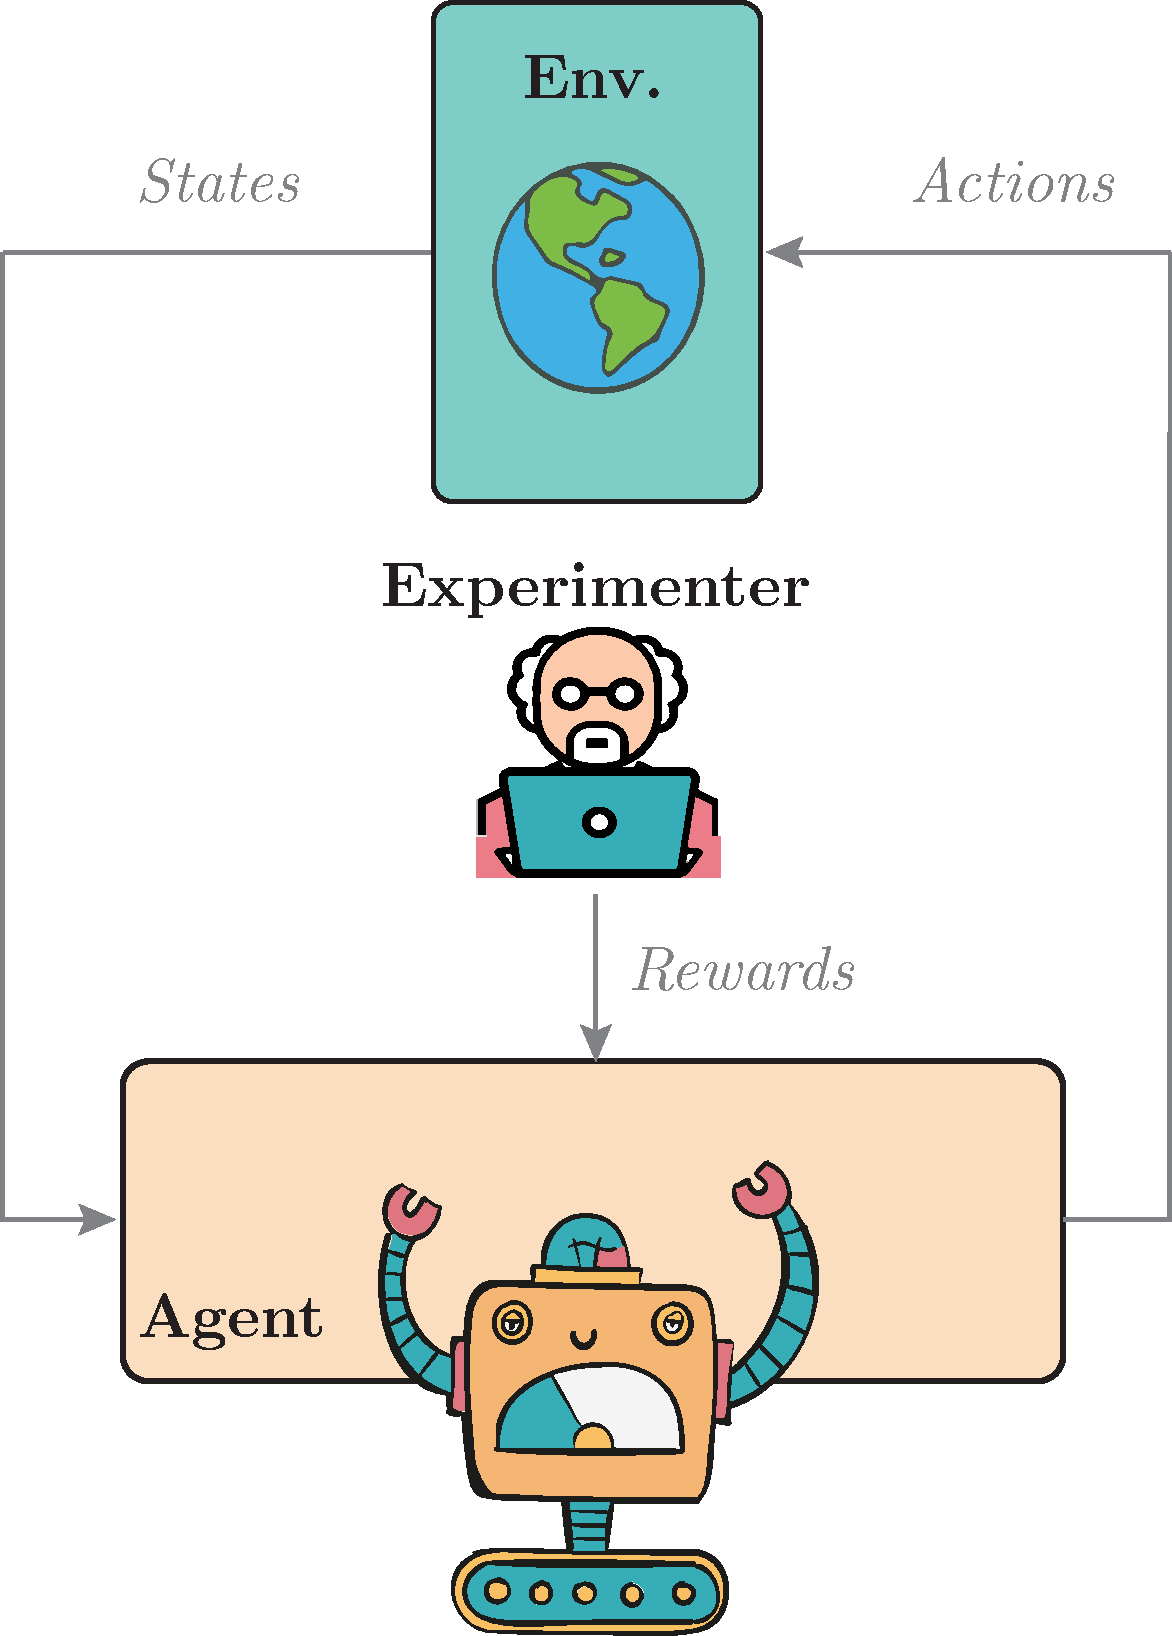
\includegraphics[width=0.3\textwidth]{background/rl_interactions.pdf}	
\caption{Interactions in a \rl loop}
\label{fig:rl_interacvtions}
\end{figure}
The transition function $\m{T}$ gives the distribution of the following states from the current state and action: $\m{T}=P_E(.|s, a)$ with $P_E$ being the (potentially stochastic) dynamics of the environment. In an \mdp, the transition function must respect the \textit{Markov property}: a future state ($s'$) must only depend on the current state ($s$) and not on its predecessor, i.e. the transition function is memoryless. 
\begin{equation}
 P_E(s_{t+1}|s_t,a_t) = P_E(s_{t+1}|s_0,\dots,s_t,a_t)	
\end{equation}

In a \rl problem, the behavior of the agent is expressed as a \textit{policy} $\pi : \m{S} \rightarrow \m{A}$ that predicts the next action $a$ based on the current state $s$. This policy can be stochastic ${a_t\sim\pi(.|s_t)}$ or deterministic $a_t=\bar{\pi}(s_t)$. When agents interact in an environment, they produce \textit{trajectories}. A trajectory is a sequence of states and actions $\tau=(s_0,a_0,\dots,s_T,a_T)$. When both the dynamics of the environment and the policy of the agent is stochastic, the probability of a trajectory is:
\begin{equation}
P(\tau|\pi)=\rho_0(s_0)\prod_{t=0}^{T-1} P_E(s_{t+1}|s_t,a_t)\pi(a_t|s_t)	
\label{eq:traj_dist}
\end{equation}
The objective of the agent is to maximize the cumulative reward computed over trajectories ($R^{tot}$). When computing the aggregation of rewards,  we often introduce discounting and give smaller weights to delayed rewards. The return of a trajectory is therefore:
\begin{equation}
R^{tot}(\tau) = \sum_{t=0}^{T} \gamma^{t}R(s_t,a_t)
\end{equation}
with $\gamma \in ]0,1]$ being a constant discount factor. We call the optimal policy $\pi^*$, the behavior that maximizes the expected return:
\begin{equation}
	\pi^*=\argmax_\pi \expect{\tau\sim\pi}[R^{tot}(\tau)] = \argmax_\pi \expect{(a_t\sim\pi, s_t\sim P_E)}\left[\sum_{t=0}^{T} \gamma^{t}R(s_t,a_t)\right]
\end{equation}
The reward function plays therefore a crucial role in a \rl problem as its maximization will directly shape the behavior of the agent.

\paragraph{Value Functions}

Most \rl algorithms rely on the definition of \textit{value} and \textit{action-value} functions:

\begin{tcolorbox}
\small
\paragraph{Definitions}
\begin{itemize}[noitemsep]
	 \item The \gls{value function} $V_\pi(s)$ of a policy $\pi$ gives the expected return of a trajectory starting from $s$ and following $\pi$. 
	 \item The \gls{action-value function} $Q_\pi(s,a)$ is the expected return of the trajectory taking action $a$ from state $s$ before following $\pi$ from the next state $s'$. 
\end{itemize}
\end{tcolorbox}
Action-value functions are powerful because they allow us to instantly assess the quality of a situation without waiting for the end of the trajectory. The value and action-value function obey the Bellman expectation equations~\citep{sutton1998intra}, a recursive definition that states that the value of a certain state (when following policy $\pi$) is equal to the sum of the instantaneous reward and the value from the next state.
\begin{equation}
\left\{
\begin{split}
	V_\pi(s) & = \underset{(a\sim\pi, s'\sim P_E)}{\mathbb{E}}\left[R(s,a) + \gamma V_\pi(s')\right]  \\
	Q_\pi(s,a) &= \underset{s'\sim P_E}{\mathbb{E}}\left[ R(s,a) + \gamma \underset{a' \sim \pi}{\mathbb{E}}[Q_\pi(s',a')]\right]
\end{split}
\right.	
\end{equation}
The value and action-value functions also follow the Bellman optimality equation where expectations over actions are replaced by max operators.
\begin{equation}
\left\{
\begin{split}
	V^*(s) & = \max_a\underset{s'\sim P_E}{\mathbb{E}}\left[R(s,a) + \gamma V^*(s')\right]  \\
	Q^*(s,a) &= \underset{s'\sim P_E}{\mathbb{E}}\left[ R(s,a) + \gamma \max_{a'}[Q^*(s',a')]\right]
\end{split}
\right.	
\end{equation}
Acting greedily with respect to the optimal action-value function gives the optimal policy:
\begin{equation}
\pi^*(s) = \argmax_a Q^*(s,a)	
\end{equation}


Computing $Q^*$ is therefore a way to solve a \rl problem. When agents have access to perfect knowledge of the dynamic of the environment ($P_E$) and when the dimensionality of $\m{S}$ and $\m{A}$ is small, they can do planning to find the optimal action-value function via Dynamic Programming~\citep{bellman1966dynamic} for instance. Planning approaches that leverage the transition function of the environments are called \textit{model-based} \rl algorithms. They are opposed to \textit{model-free} \rl algorithms that do not use $P_E$ but interact directly with a simulator (with transition function $P_S$).

Because the present research builds on both families of solutions, we detail the techniques used for each in the following paragraphs. We first briefly detail the \textit{Monte-Carlo Tree Search} planning algorithm (\mcts)~\citep{browne2012mcts} used in our first experimental contribution (in chapter~\ref{chap:abig}) and then introduce the deep \rl algorithm used in chapter~\ref{chap:imagine}.

\paragraph{Model-based \rl with \mcts:}

\mcts is a tree-search algorithm that seeks to identify the optimal policy by finding the action with the highest Q-value. To this end, \mcts build an estimate $\hat{Q}(s,a)$ for $a \in \m{A}$ in a given state $s$ and acts greedily with respect to this estimate. Each node of the tree is a state $s$ while edges are the potential actions. The \mcts algorithm grows the tree iteratively using an exploration/exploitation tradeoff to efficiently refine $\hat{Q}$ in promising regions of the \mdp. More specifically, each iteration of the \mcts algorithm contains four steps:
\begin{enumerate}[noitemsep]
	\item \textbf{Selection:} In the selection phase, the \mcts algorithm starts from the root node and uses a tree policy to decide which node to expand. The tree policy is guided by an evaluation function ($UCT$) and stops when a node with remaining actions to explore is reached. 
	\item \textbf{Expansion:} Once a leaf node is reached, a new action $a$ is sampled among the non-explored ones and the corresponding node is computed using the transition function $s' \sim P_E(.|s,a)$
	\item \textbf{Simulation:} From the newly created node corresponding to state $s'$, a simulation policy $\pi_{sim}$ is used to draw a full trajectory (until termination or for a predefined horizon) and compute return $R^{tot}$. $\pi_{sim}$ is often a random policy.
	\item \textbf{Backpropagation:} $R^{tot}$ is backpropagated to the root node as indicated in \fig{fig:mcts_steps}.
\end{enumerate}
For the tree policy evaluation function, we use the Upper Confidence Bound~\citep{auer_finite-time_2002}: $UCT = \frac{1}{k}\sum_{i=0}^{k} R^{tot}_{i} + C\sqrt{\frac{\text{ln}(n)}{k}}$ where $k$ is the number of completed trajectory going through node $s$ and $n$ is the number of iterations. The first term of $UCT$ is an estimation of the expected return while the second term encourages the tree policy to explore unexpanded nodes.
\begin{figure}[!h]
\centering
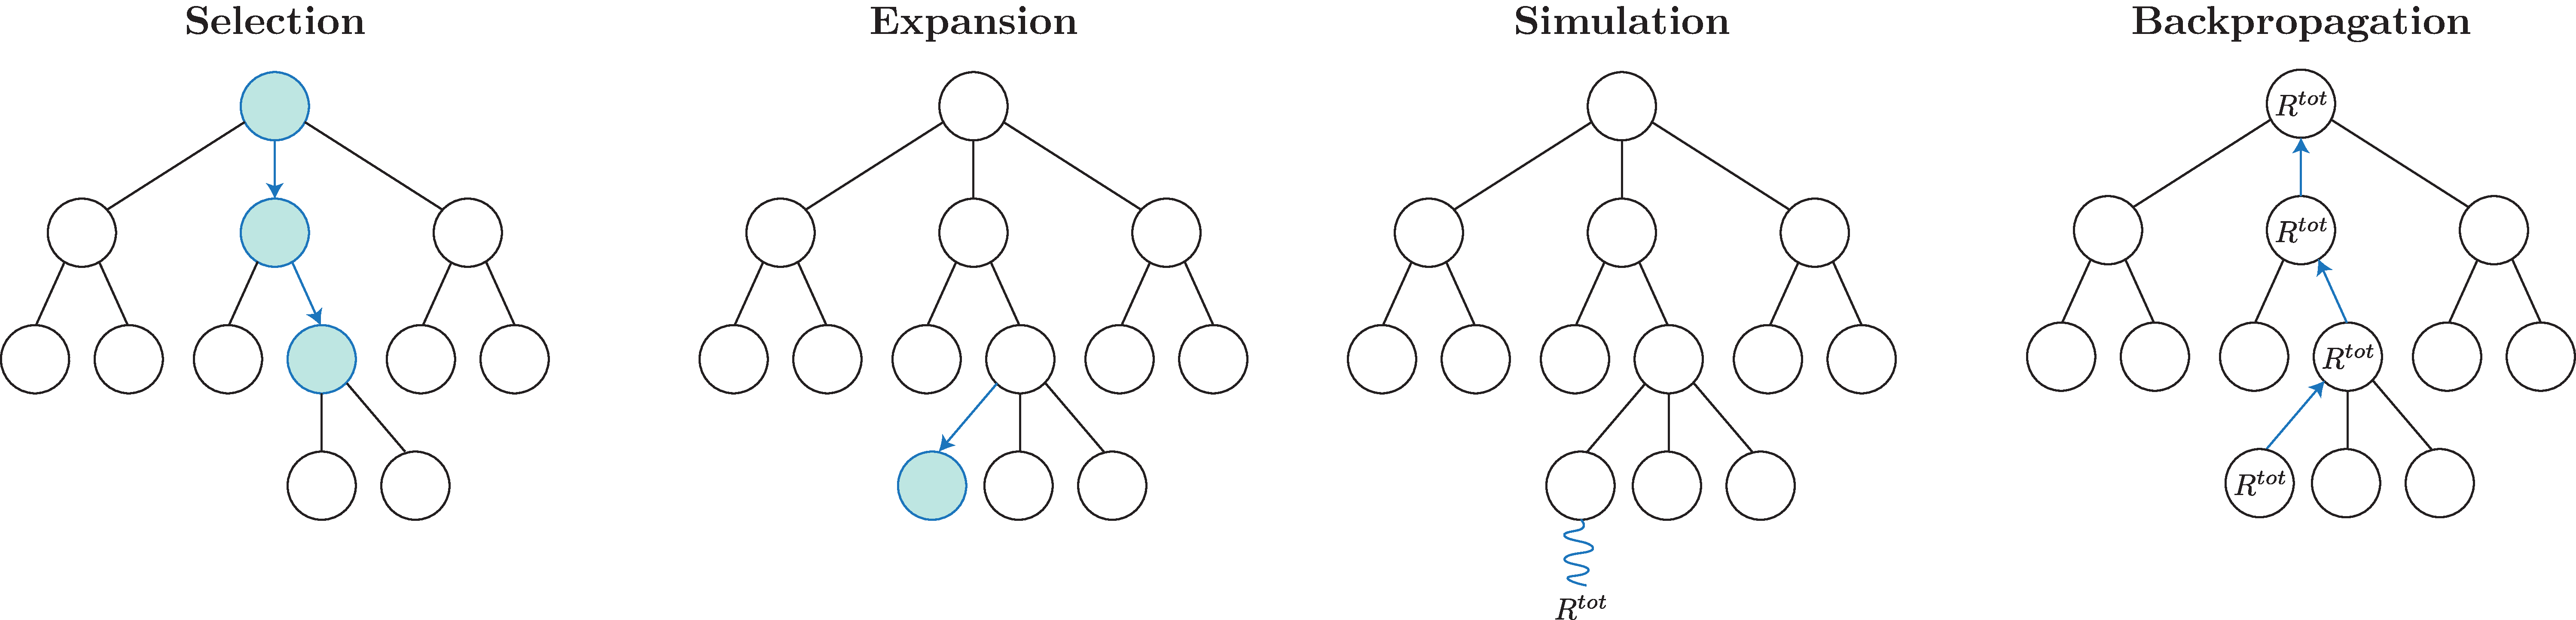
\includegraphics[width=1\textwidth]{background/mcts_4_steps.pdf}
\caption{The four steps of an \mcts iteration}
\label{fig:mcts_steps}	
\end{figure}

\paragraph{Model-free \rl with Q-learning:}

Some of the experimental contributions of this research build on the \textit{Deep Deterministic Policy Gradient} (\ddpg) algorithm~\citep{lillicrap2015continuous}. \ddpg derives from \textit{Deep Q-Networks} (\dqn) \citep{mnih2015human} which is itself a deep learning implementation of the standard \textit{Q-learning} algorithm~\citep{watkins_q-learning_1992}.  In this paragraph, we propose to detail the steps that allow building DDPG from Q-learning. 

\textbf{Q-learning} is an \textit{off-policy} \rl algorithm. Off-policy algorithms, in contrast to on-policy algorithms, learn to approximate the action-value $Q^*$ of an optimal policy independently of the policy used for data collection. Q-learning relies on transitions $(s,a,r,s')$ collected by a policy $\pi_c$ interacting with a simulator $P_S$. Assuming that $Q$ is a linear combination of features ($\phi$): $Q(s,a;\theta)=\theta^T\phi(s,a)$, the algorithm iteratively learns to approximate $Q^*$ by minimizing the temporal difference error (TD-error):
\begin{equation}
\m{L}_i=\underset{(s\sim P_S, a\sim\pi_c)}{\mathbb{E}} \left[(y_i - Q(s,a;\theta_i))^2 \right] \text{ with } y_i = \underset{s'\sim P_S}{\mathbb{E}}\left[r +\gamma \max_{a'}Q(s',a';\theta_{i-1})\right] 
\label{eq:loss_td}
\end{equation}
In the original formulation of the Q-learning algorithm by \citet{watkins_q-learning_1992}, they consider a tabular setting and store the Q-values at each iteration in a table ($Q_i[s,a]$) instead of using linear function approximations. The update of the table writes:
\begin{equation}
Q_{i+1}[s,a] \leftarrow Q_i[s,a] + \alpha \left(r + \gamma\max_{a'}Q_i[s',a'] - Q_i[s,a]\right)
\end{equation}


\textbf{\dqn} proposes to represent the action-value function with deep neural networks: $Q(s,a;\theta)$ with parameters $\theta$. The architecture of the network takes a state $s$ as input and outputs the value of each action $Q(s,a) \forall a \in \mathcal{A}$. Thus \dqn only works with discrete action space. When differentiating \eq{eq:loss_td} with respect to the neural network parameters, we get:
\begin{equation}
	\nabla_{\theta_i }\m{L}_i(\theta_i ) = \underset{(s\sim P_S, a\sim\pi_c)}{\mathbb{E}} \left[(y_i - Q(s,a;\theta _i))\nabla_{\theta_i }Q(s,a;\theta _i)\right]
\end{equation}
During differentiation, one has to pay particular attention to freezing the weights of the network when evaluating $y_i$. Deep neural networks are known to exhibit training instabilities. In order to stabilize learning, \citet{mnih2015human} proposed two main innovations: 
\begin{itemize}[noitemsep]
\item \textit{Experience Replay}: The agent uses a replay buffer to store transitions during interactions. During learning, the transitions are then sampled uniformly to perform updates. This enables breaking the correlation between successive transitions and reusing them.
\item \textit{Target network}: A target network is used to compute target $y$. This network is initialized with the actual Q-network ($Q_{targ}(s,a;\theta_{targ})=Q(s,a;\theta$) but updated less frequently than the actual Q-network. Updates are often performed using \textit{Polyak averaging}~\citep{polyak1992}: $\theta_{targ} \leftarrow \rho\theta_{targ} + (1-\rho)\theta$ with $\rho$ being the polyak factor.
\end{itemize}

\textbf{\ddpg} is an adaptation of \dqn to continuous action space. The challenge of dealing with continuous actions is to act greedily with respect to the learned Q-value. i.e. to evaluate $\argmax_a Q(s,a)$. To overcome this, \ddpg concurrently learns a deterministic policy with the Q-function. This policy is a parametrized network $\pi(s;\phi)$ with parameters $\phi$ and is obtained by gradient ascent. Moreover, since $\pi(s;\phi) \approx \argmax_a Q(s,a,\theta)$ it can be injected in \eq{eq:loss_td}. We, therefore, have the two following losses to optimize:
\begin{equation}
\left\{
\begin{split}
	\m{L}_{\pi_\phi} &= \underset{(s\sim P_S)}{\mathbb{E}}\left[Q_\theta(s,\pi_\phi(s))\right] \quad \quad \quad \quad \text{ (Policy loss)}\\
	\m{L}_{Q_\theta} &= \underset{(s\sim P_S,a\sim\pi_c)}{\mathbb{E}}\left[(y- Q_\theta(s,a))^2 \right] \quad \text{(Q-value loss)}\\
	& \text{with } y = \underset{s'\sim P_S}{\mathbb{E}}\left[r +\gamma Q_\theta(s',\pi_\phi)\right]
\end{split}
\right.
\end{equation}
where parameter dependencies have been subscripted.

\paragraph{Other model-free \rl algorithms}

There are numerous algorithms within the field of \drl, including on-policy methos like \textsc{trpo}~\citep{pmlr-v37-schulman15}, \textsc{ppo}~\citep{ppo2017} as well as more advanced off-policy approaches like \textsc{td3}~\citep{pmlr-v80-fujimoto18a} and \textsc{sac}~\citep{pmlr-v80-haarnoja18b}.


\subsection{Imitation Learning}

\paragraph{Problem}

\textit{Imitation Learning} (\il)~\citep{pommerleau1988BC,schaal1996learning,osa2018algorithmic} is a field that considers an agent learning in a \mdp in which the reward function is not explicitly defined, but where the agent can observe demonstrations of the task it is intended to perform. \il is particularly useful in situations where it is difficult for the experimenter to design a task-specific reward function, but demonstrations are available. A classic example from the literature is the application of \il to self-driving cars. It is impractical to specify a reward function for the task of driving as successful drivers constantly adjust their criteria to adapt to the various events that occur on the road. However, there is a vast amount of video footage of people driving that could potentially be utilized by the agent to learn.

\begin{figure}[!h]
\centering
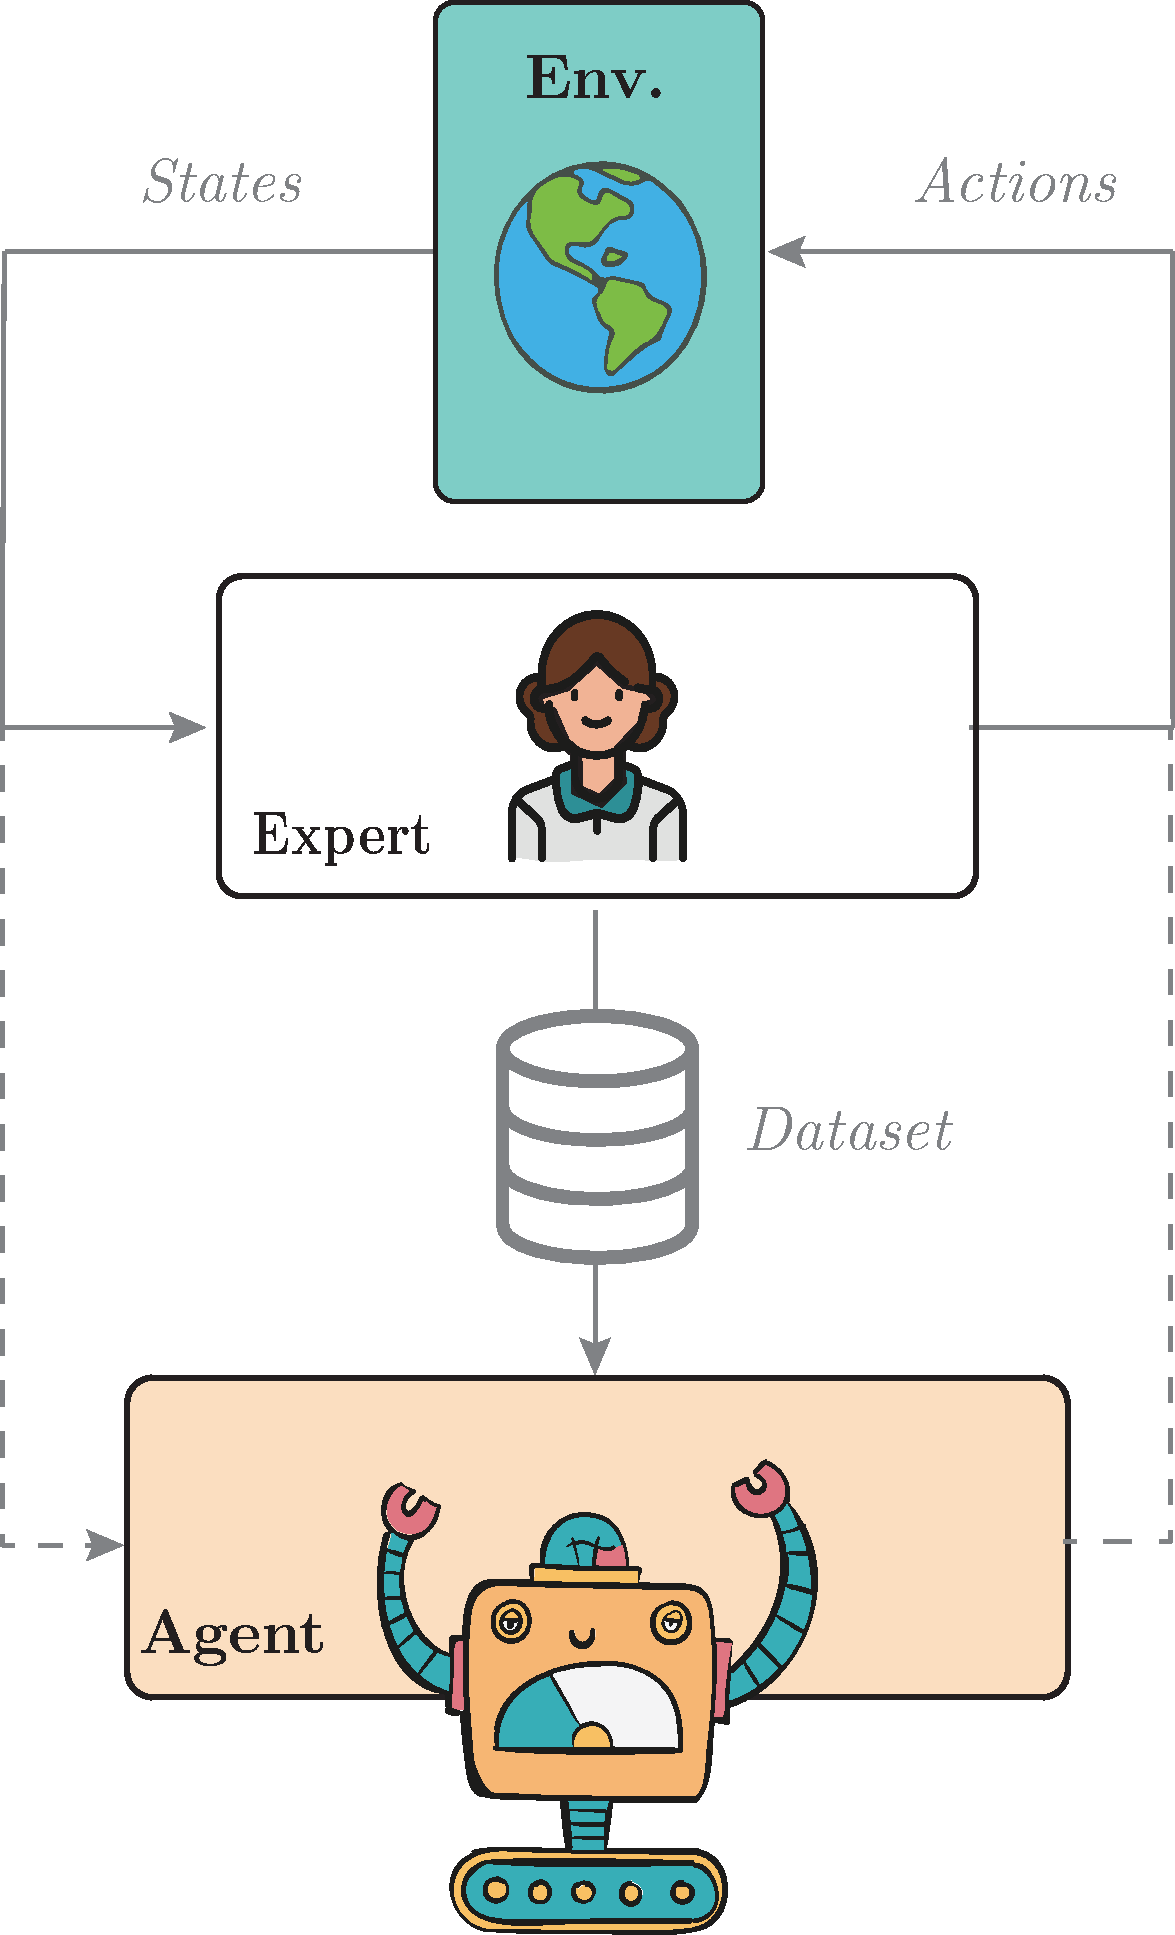
\includegraphics[width=0.3\textwidth]{background/il_interactions.pdf}	
\caption{Interactions in a \il problem. The agent never interacts with the environment during learning but can interact with it to test its behavior (dashed lines).}
\label{fig:il_interacvtions}
\end{figure}

A standard way of formalizing the \il problem is to find a policy that minimizes the divergence between the expert and learner data distribution. Provided a dataset $\m{D}=\{(\tau_i)\}_{i=1}^N$ containing expert trajectories of features $\tau = [\phi_0,\dots, \phi_T]$. If $q_{\pi^*}(\phi)$ is the distribution of features induced by the expert's policy (supposed optimal $\pi^*$) and $p_\pi(\phi)$ is the distribution of features induced by the learners' policy ($\pi$), the goal of \il is to find policy $\hat{\pi}$ such that:
\begin{equation}
\hat{\pi} = \argmin_{\pi}D(q_{\pi^*}(\phi),p_\pi(\phi))
\end{equation}
with $D$ being a measure of differences between probability distributions such as the well-known Kullback-Leibler (KL) divergence.

\paragraph{Behavioral Cloning}

An intuitive way of solving an \il problem is to frame it as a supervised learning setting and do \textit{Behavioral Cloning}(\bc). Given a dataset of trajectories $\m{D}=\{(\tau_i)\}_{i=1}^N$ with  $\tau=[(s_0,a_0) \dots (s_T,a_T)]$, one directly minimizes the cross entropy loss:
\begin{equation}
\m{L}_\pi = -\expect{(s,a)~\sim\m{D}}[\log\pi(s,a)]
\end{equation}
Minimizing this cross-entropy loss is in fact equivalent to minimizing the KL-divergence between the trajectory distribution of the expert $P(\tau|\pi^*)$ and the trajectory distribution of the learner $P(\tau|\pi)$~\citep{ke2020imitation}:
\begin{equation}
D_{KL}(P(\tau|\pi^*),P(\tau|\pi)) = \underset{\tau \in \m{D}}{\sum}P(\tau|\pi^*)\log\left(\frac{P(\tau|\pi^*)}{P(\tau|\pi)}\right)
\end{equation}
%
Injecting the definition of the trajectory distribution of \eq{eq:traj_dist} we get that:
%
\begin{align}
D_{KL}(P(\tau|\pi^*),P(\tau|\pi)) &= \underset{\tau \in \m{D}}{\sum}P(\tau|\pi^*)\log\left(\prod_{t=0}^{T-1}\frac{\pi^*(a_t|s_t)}{\pi(a_t|s_t)}\right) \\
&= \underset{\tau \in \m{D}}{\sum}P(\tau|\pi^*)\sum_{t=0}^{T-1}\left(\log\pi^*(a_t|s_t) - \log\pi(a_t|s_t)\right) \\
&= \expect{(s,a)\sim\m{D}}\left[\log\pi^*(a_t|s_t) - \log\pi(a_t|s_t)\right]
\end{align}
%
We will use behavioral cloning in chapter~\ref{chap:abig}. \bc is a straightforward method for reproducing expert behavior. However, simple \bc only works if the agent operates in the same region of the state space as the states provided in $\m{D}$. Otherwise, the policy of the learner will progressively deviate from this region accumulating errors at each time step. This compounding error is called \textit{distributional mismatch}. One way of addressing it is to iteratively collect new expert data when needed (in the initially uncovered region of the state space)~\citep{dagger2011}. 

Another limitation of \bc is that it is only able to derive an optimal policy from optimal expert trajectories, meaning that the learned policy will not exceed the performance of the expert. In some applications collecting optimal trajectories is not always possible. As a result, some researchers have turned to \textit{Inverse Reinforcement Learning} (\irl) as an alternative approach.

\paragraph{Inverse Reinforcement Learning}

Similar to \rl, \irl can be understood both as a problem and a category of techniques. The \irl problem consists in recovering the reward function of an expert given a dataset of its trajectories~\citep{ng2000irl}. As such \irl algorithmic solutions followed by \rl can form a solution to the \il problem. The combination of \irl followed by \rl is called \textit{Apprenticeship Learning}~\citep{abbeel2004apprenticeship}. As opposed to \bc, apprenticeship learning ensures that the learned policy is bellman consistent (with respect to an underlying learned value-function). As formalized by \citet{klein2011apprenticeship}, there are mainly three categories of strategies to obtain the policy:
\begin{enumerate}[noitemsep]
\item Feature-expectation-based methods as proposed by \citet{ziebart2008maxentirl} which learn a reward function such that the feature expectation of the optimal policy (according to the learned reward function) is similar to the feature expectation of the expert policy. 
\item Margin-maximization-based methods~\citep{ratlif2006maxmargin}, which formulate \irl as a constrained optimization problem in which the expert's examples have a higher expected cumulative reward than all other policies by a certain margin.
\item Approaches based on the parameterization of the policy by the reward~\citep{neu2007apprenticeship}: If it is assumed that the expert follows a Gibbs policy (or the optimal value function related to the optimized reward function), it is possible to estimate the likelihood of a set of state-action pairs provided by the expert.
\end{enumerate}
%
Recent feature-expectation-based approaches use technics similar to generative adversarial networks (\gan)~\citep{goodfellow2014generative} to imitate complex behavior in high-dimensional environments~\citep{ho2016gail}. Other approaches use ranking of trajectories to reach better-than-demonstrator performances~\citep{brown2020better}. As we do not leverage \irl in our contributions we will not detail these methods (see \citet{arora_survey_2021} for a thorough survey of \irl algorithms).


\subsection{Muli-Goal Reinforcement Learning}
\label{sec:background_mg_rl}
Standard \rl can be extended to a multi-goal setting. Let us return to the definition of goal by \citet{elliot2008goal} provided in the introduction (\sect{sec:humans_autotelic}):
\begin{quote}
   	``\textit{A goal is a cognitive representation of a future object that the organism is committed to approach or
    avoid} ''.
\end{quote}
\rl algorithms seem, indeed, to be a good fit to train goal-conditioned agents: they train learning agents (\textit{organisms}) to maximize (\textit{approach}) a cumulative (\textit{future}) reward (\textit{object}). In \rl, goals can be seen as a set of \textit{constraints} on one or several consecutive states that the agent seeks to respect. These constraints can be very strict and characterize a single target point in the state space (\eg image-based goals) or a specific sub-space of the state space (\eg target x-y coordinate in a maze, target block positions in manipulation tasks). They can also be more general when expressed by language for example (\eg '\textit{find a red object or a wooden one}'). 

\paragraph{Formal Definition of Goals and Skills}

To represent these goals, \rl agents must be able to 1)~have a compact representation of them and 2)~assess their progress towards it. This is why we propose the following formalization for \rl goals: 

\begin{tcolorbox}
\small
\paragraph{Generalized definition of the goal construct for \rl:}
\begin{itemize}
    \item \gls{Goal}: a $g\,=\,(z_g,\,R_g)$ pair where $z_g$ is a compact \textit{goal parameterization} or \textit{goal embedding} and $R_g$ is a \textit{goal-achievement} function.
    \item \gls{Goal-achievement function}: $R_g(\cdot)\,=\,R_\m{G}(\cdot\mid\,z_g)$ where $R_\m{G}$ is a goal-conditioned reward function.
\end{itemize}
\end{tcolorbox}

The objective of a goal-conditioned agent is to learn a \textit{goal-conditioned policy}: a function that generates the next action given the current state and the goal $a_t \sim \pi(\cdot|s_t,z_g)$. The goal-achievement function and the goal-conditioned policy both assign \textit{meaning} to a goal. The former defines what it means to achieve the goal, it describes how the world looks like when it is achieved. The latter characterizes the process by which this goal can be achieved; what the agent needs to do to achieve it. In this search for the meaning of a goal, the goal embedding can be seen as the map: the agent follows this map and via the two functions above, experiences the meaning of the goal.

\begin{tcolorbox}
\small
\paragraph{Definition}
\begin{itemize}
    \item \gls{Goal-conditioned policy}: a function that generates the next action given the current
state and the goal.
	\item \gls{Skill}:  the association of a goal and a policy to reach it.
\end{itemize}
\end{tcolorbox}

\paragraph{Problem}

By replacing the unique reward function $R$ by the space of reward functions $\m{R}_\m{G}$ in the definition of \mdp of \eq{eq:standard_mdp}, \rl problems can be extended to handle multiple goals: $\m{M}\,=\,\{\m{S},\,\m{A},\,\m{T},\,\rho_0,\,\m{R}_\m{G}\}$. The term \textit{goal} should not be mistaken for the term \textit{task}, which refers to a particular \mdp instance. As a result, \textit{multi-task} \rl refers to \rl algorithms that tackle a set of \mdps that can differ by any of their components (\eg $\m{T}$,\,$R$,\,$\rho_0$, etc.). The \textit{multi-goal} \rl problem can thus be seen as the particular case of the multi-task \rl problem where \mdps differ by their reward functions. In the standard multi-goal \rl problem, the set of goals\,---\,and thus the set of reward functions\,---\,is pre-defined by engineers. As one can observe in \fig{fig:mg_rl_interactions}, the experimenter sets goals to the agent, and provides the associated reward functions. 


\begin{figure}[!h]
\centering
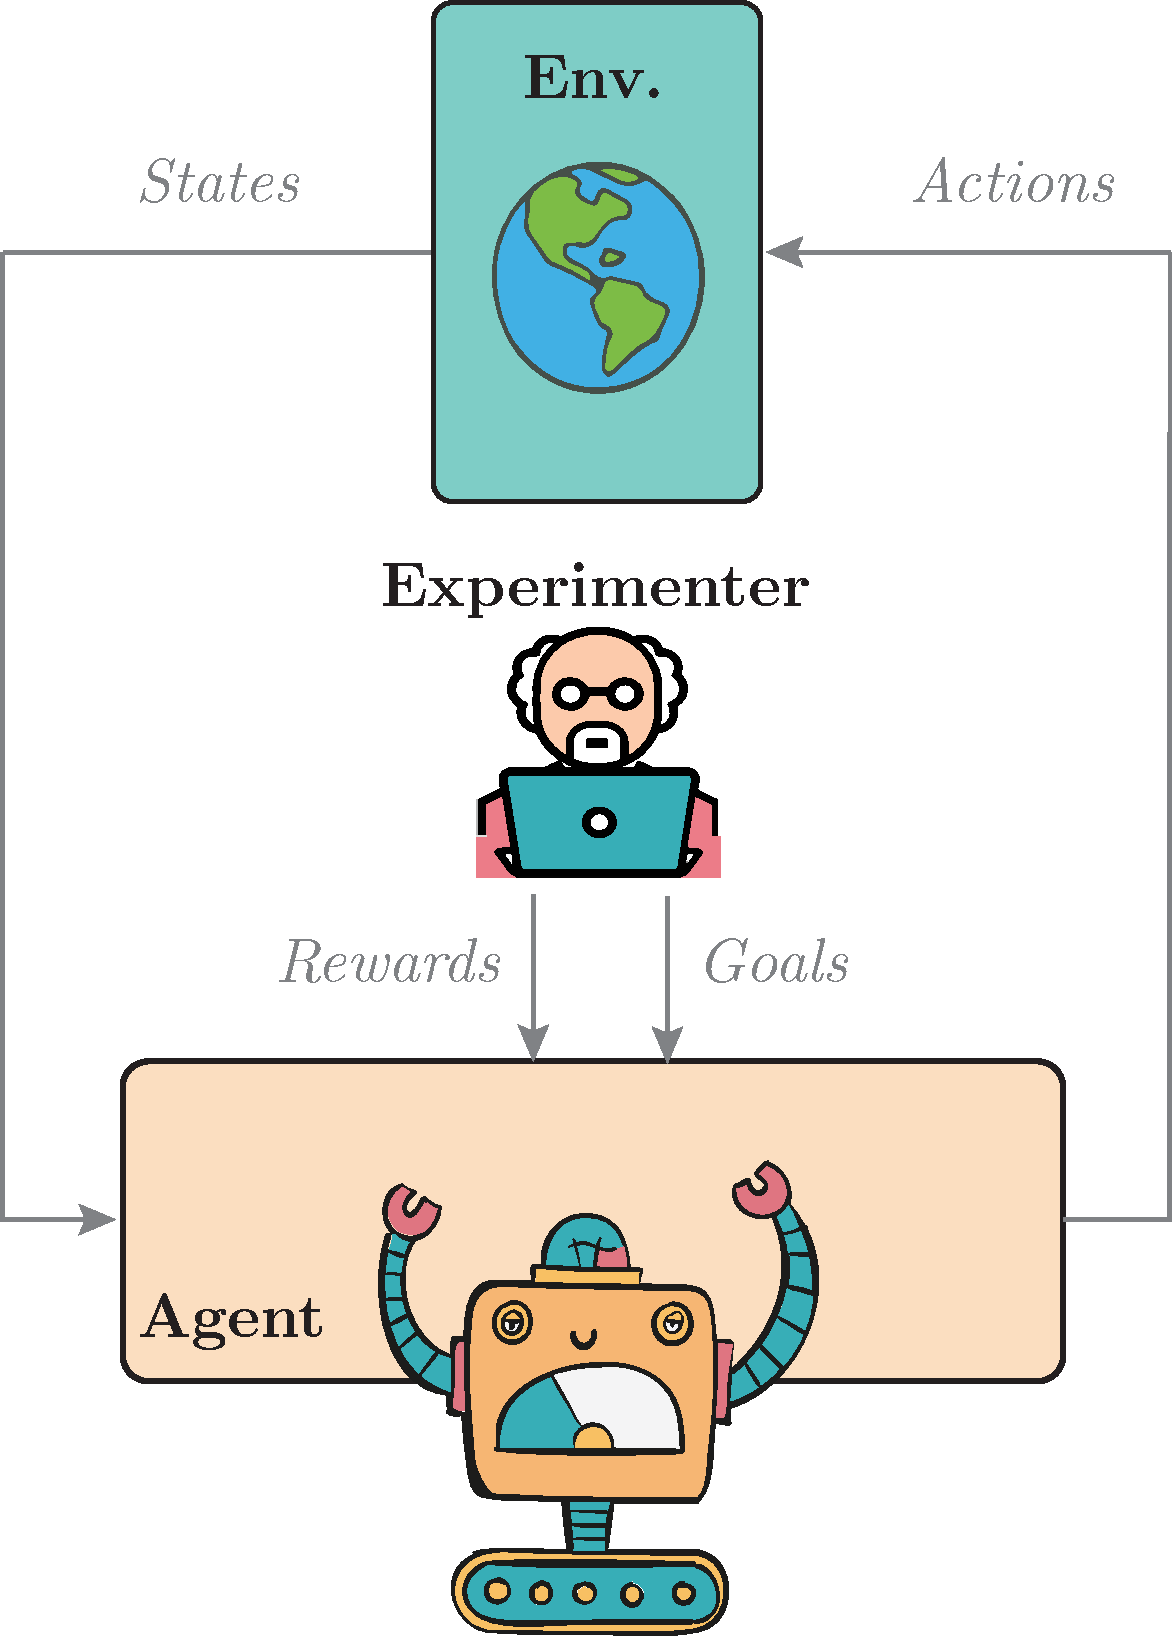
\includegraphics[width=0.3\textwidth]{background/multi_goal_rl_interactions.pdf}	
\caption{Interactions in a multi-goal \rl loop. The experimenter provides goals and their associated rewards to the agent.}
\label{fig:mg_rl_interactions}
\end{figure}


\paragraph{Solutions: Horde, UVFA, and HER}

Goal-conditioned agents see their behavior affected by the goal they pursue. This is formalized via goal-conditioned policies, that is policies that produce actions based on the environment state and the agent's current goal: 
\begin{equation}
\Pi:\m{S}\times\m{Z}_\m{G}\to\m{A}
\end{equation}
where $\m{Z}_\m{G}$ is the space of goal embeddings corresponding to the goal space $\m{G}$~\citep{schaul2015universal}. Note that ensembles of policies can also be formalized this way, via a meta-policy $\Pi$ that retrieves the particular policy from a one-hot goal embedding $z_g$~\citep{kaelbling1993learning,sutton2011horde}.

The idea of using a unique \rl agent to target multiple goals dates back to \citep{kaelbling1993learning}. Later, the \horde architecture proposed to use interaction experience to update one value function per goal, effectively transferring to all goals the knowledge acquired while aiming at a particular one \cite{sutton2011horde}. In these approaches, one policy is trained for each of the goals and the data collected by one can be used to train others.

Building on these early results, \citet{schaul2015universal} introduced \textit{Universal Value Function Approximators} (\uvfa). They proposed to learn a unique goal-conditioned value function and goal-conditioned policy to replace the set of value functions learned in \horde. Using neural networks as function approximators, they showed that \uvfas enable transfer between goals and demonstrate strong generalization to new goals.

The idea of \textit{hindsight learning} further improves knowledge transfer between goals~\citep{kaelbling1993learning,andrychowicz2017hindsight}. Learning by hindsight, agents can reinterpret a past trajectory collected while pursuing a given goal in the light of a new goal. By asking themselves, \textit{what is the goal for which this trajectory is optimal?}, they can use the originally failed trajectory as an informative trajectory to learn about another goal, thus making the most out of every trajectory~\citep{eysenbach2020rewriting}. This ability dramatically increases the sample efficiency of goal-conditioned algorithms and is arguably an important driver of the recent interest in goal-conditioned \rl approaches.


\subsection{Multi-Agent Reinforcement Learning}
\label{sec:background_marl}
\paragraph{Problem}

Standard \rl can also be extended to scenarios where several agents interact with the environment. For this purpose \mdps are extended to \textit{Markov Games}.
\begin{tcolorbox}
\small
\paragraph{Definition}
\gls{Markov Game} are defined by the following terms:
\begin{equation}
	\m{M}\,=\,\{\m{S},\m{T},\,\rho_0,\,\{\m{O}_i,\m{A}_i,R_i\}_{i=1}^N\}
	\label{eq:markov_game}	
\end{equation}
The first three terms of a Markov Game are the same as those of a \mdp: $\m{S}$ is the state space, $\m{T}$ is the transition function, and $\rho_0$ the initial state distribution. However, each agent (denoted by the index $i$) perceives a different perspective of the state through observation transformation $\m{O}_i$. Agents also have different action spaces $\m{A}_i$ and reward function $R_i$
\end{tcolorbox}

In Multi-Agent Reinforcement learning (\marl), each agent aims at learning a policy that maps their observation $o_i=\m{O}_i(s)$ to actions: $a_i \sim \pi_i(\cdot|o_i)$. Similarly to \rl, each agent aim at maximizing its expected return:
\begin{equation}
	\pi_i^* = \argmax_{\pi_i} \expect{(a_t\sim\pi_i, s_t \sim P_E}\left[\sum_{t=0}^T\gamma^tR_i(\m{O}_i(s_t),a_t)\right]
\end{equation}
A diagram of interaction is provided in \fig{fig:marl_interactions}. The field of \marl considers mainly two types of tasks:
\begin{itemize}[noitemsep]
\item \textit{Cooperative tasks} where the agents pursue the same goal and need to coordinate in order to solve it. Cooperative tasks are usually hard to design and often involve the maximization of a common objective (sometimes at the expense of individual gains). For a review of cooperative \marl see~\citet{OroojlooyJadid2019cooperative}.
\item \textit{Competitive tasks} where the agents pursue non-aligned goals. In these settings agents explicitly aim at maximizing their individual gains. 
\end{itemize}
Among the recent innovations in \marl, \citet{Baker2020Emergent} trained agents to play the hide-and-seek game, \citet{perolat2017commonpool} to solve common-pool resource problems, and more recently \citet{team2021open} trained an agent on a spectrum of cooperative and competitive tasks including cooperative games to find objects, hide and seek or even capture the flag.

\begin{figure}[!h]
\centering
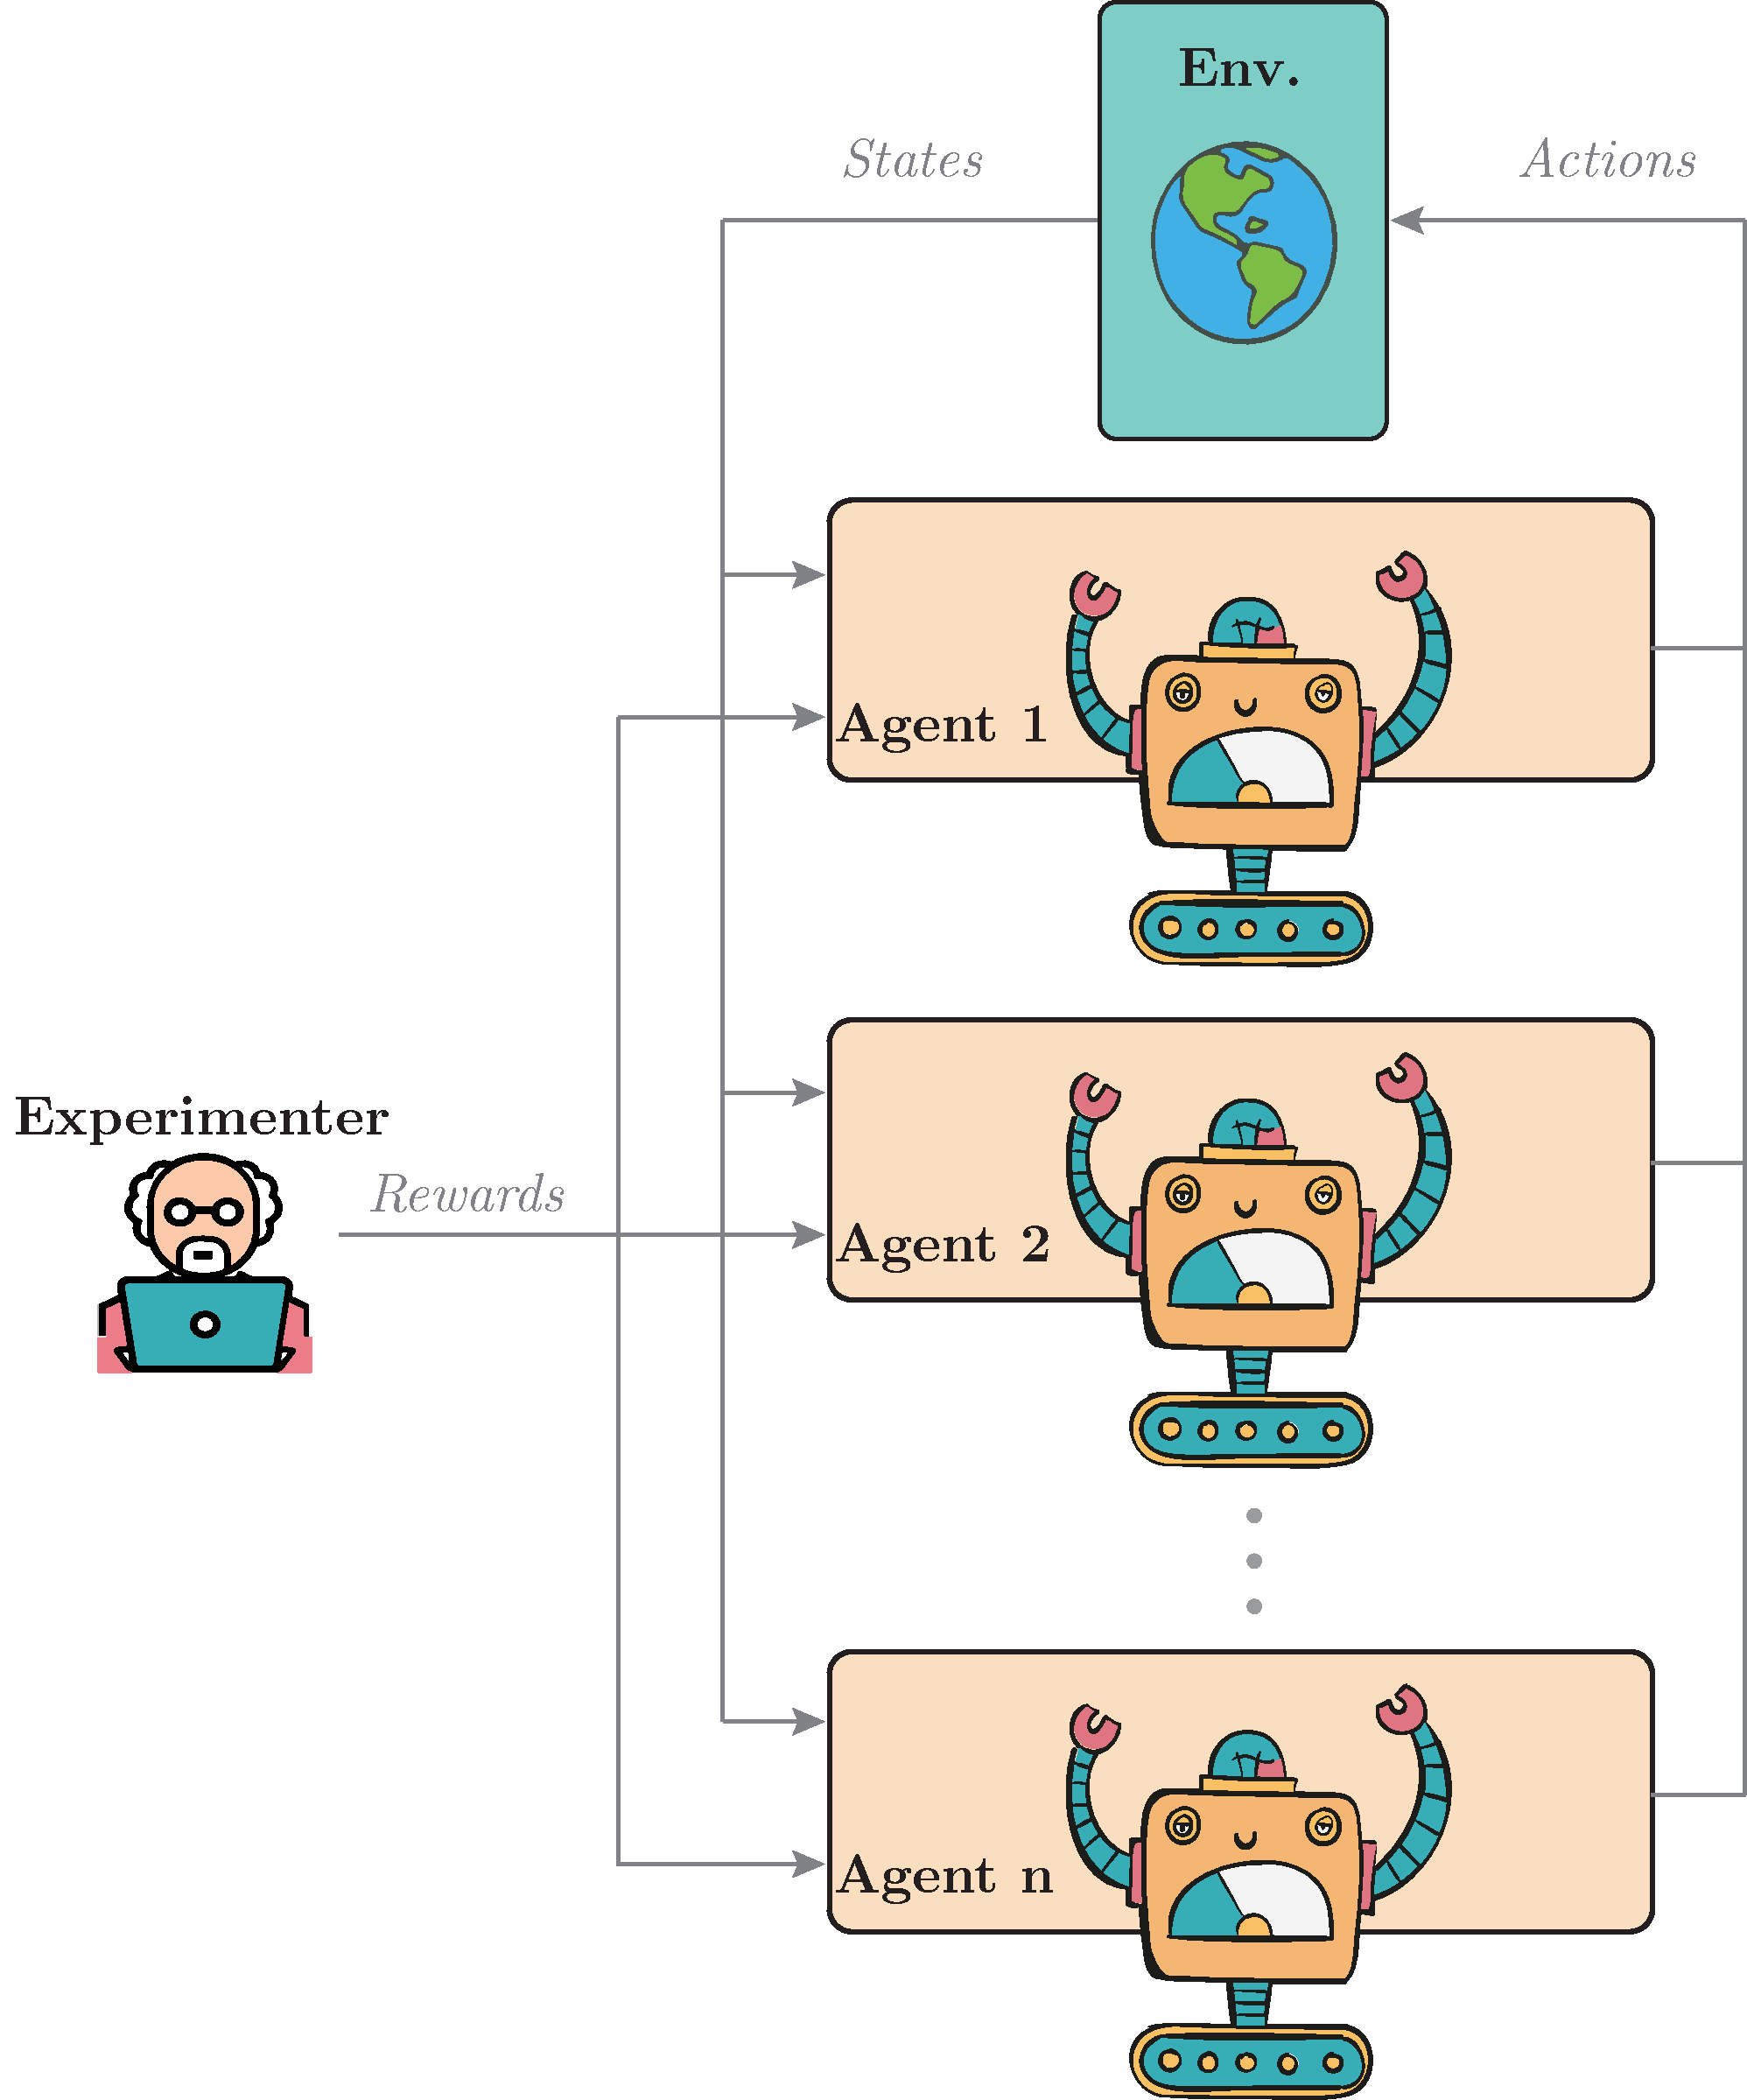
\includegraphics[width=0.5\textwidth]{background/marl_interactions.pdf}	
\caption{Diagram of interactions in a \marl loop. Each agent perceives a (potentially) different perspective of the states provided by the environment. Each agent also has its own action space and is given a (potentially) different reward.}
\label{fig:marl_interactions}
\end{figure}

\paragraph{Solution}

One of the main challenges of multi-agent learning systems is to take into account the non-stationary dynamics caused by the change of state of the agents when they learn. Indeed, an isolated agent of a Markov game does not evolve in a stationary \mdp because all agents are learning, and their behavior will be different during training. For this reason, most of the \marl algorithms rely on the \textit{centralized training, decentralized execution} paradigm. For instance, Muli-Agent Deep Deterministic Policy gradient~\citep{lowe2017multi}, uses a centralized training procedure where all agents can see other agents' observations and actions to learn an action-value function that is then used to optimize decentralized policies that only depends on local observations. As none of our contributions builds on \marl we will not elaborate on other \marl algorithms.

\newpage

\section{Problem Definition: Developmental AI}

The present research expands upon the standard \ai methods presented in previous section, with the aim of investigating fundamental inquiries within the domain of \gls{Developmental Artificial Intelligence}. Developmental \ai is a multidisciplinary field that integrates principles from artificial intelligence, developmental psychology, and neuroscience to simulate and analyze the cognitive mechanisms of artificial agents. While standard \ai paradigms are structured around precise and formal problems addresed by algorithmic contributions, developmental \ai is concerned with modelling the cognitive, sensorimotor and social development of agents. In this research the specific questions that we investigate are: 1) How do cultural conventions emerge through interactions among agents in social contexts? 2) How can embodied agents utilize cultural conventions to acquire open-ended skill repertoires? These questions can be approached through the lens of self-organization theory. Specifically, this study will examine: 1) the self-organization of conventions, or language, among agents, and 2) the role of cultural conventions in the self-organization of agents' developmental trajectories. Before introducing these two questions we will therefore define the concept of self-organization and present the challenges inherent in the field of developmental \ai.

\paragraph{Self-organization}

Self-organization is a term now used in a variety of sciences that can be described with the following definition:
\begin{tcolorbox}
\small
\paragraph{Definition}
\gls{Self-organization} is a process by which spontaneously ordered patterns and structures emerge from the interactions of the many constituents of a system without the need for central control or external guidance. Crucially, the emergent global structure of self-organizing systems cannot be explained by the properties of its constituents and must be analyzed as a whole.
\end{tcolorbox}

The notion of \textit{emerging order} draws its origin from the study of chaos and was originally used to describe thermodynamical systems that spontaneously organize themself from complex chaotic interactions. The theory of self-organization was formalized by cybernetician \citet{ashby1962self}. Borrowing concepts from dynamical system theory, he stated that any complex dynamical systems organize themselves around specific 'attractors' within a vast landscape of possible states. These attractors are stable equilibrium points and may be multiple for a given system. An intuitive explanation of attractors, proposed by \citet{dilts1995nlp}, is given in \fig{fig:youngoldlady}. It illustrates how our complex perception system can fall into different attractors when presented with an illusion. In one case, we see a young woman wearing a necklace looking up to the left, in the other we perceive an old woman leaning slightly forward. This illustration also demonstrates that certain attractors may be difficult to reach. Indeed, when looking at \fig{fig:youngoldlady} we often rapidly converge to one attractor and have difficulty escaping it to organize our perception around the other. Finding an attractor requires exploring the landscape of possible states. For this, noise and stochasticity can help as described by \citet{vonFoerster2003}:
\begin{quote}
   	``\textit{I think it is favorable to have some noise in the system. If a system is going to freeze into a particular state, it is inadaptable and this final state may be altogether wrong. It will be incapable of adjusting itself to something that is a more appropriate situation.}''
\end{quote}
\begin{figure}[!h]
\centering
\begin{tabular}{cc}
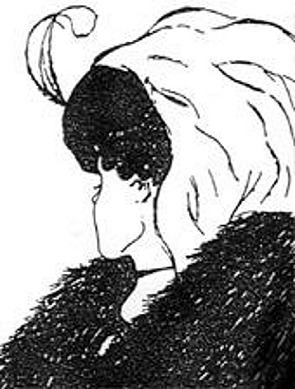
\includegraphics[width=.2\textwidth]{background/Youngoldwoman.jpg}	& 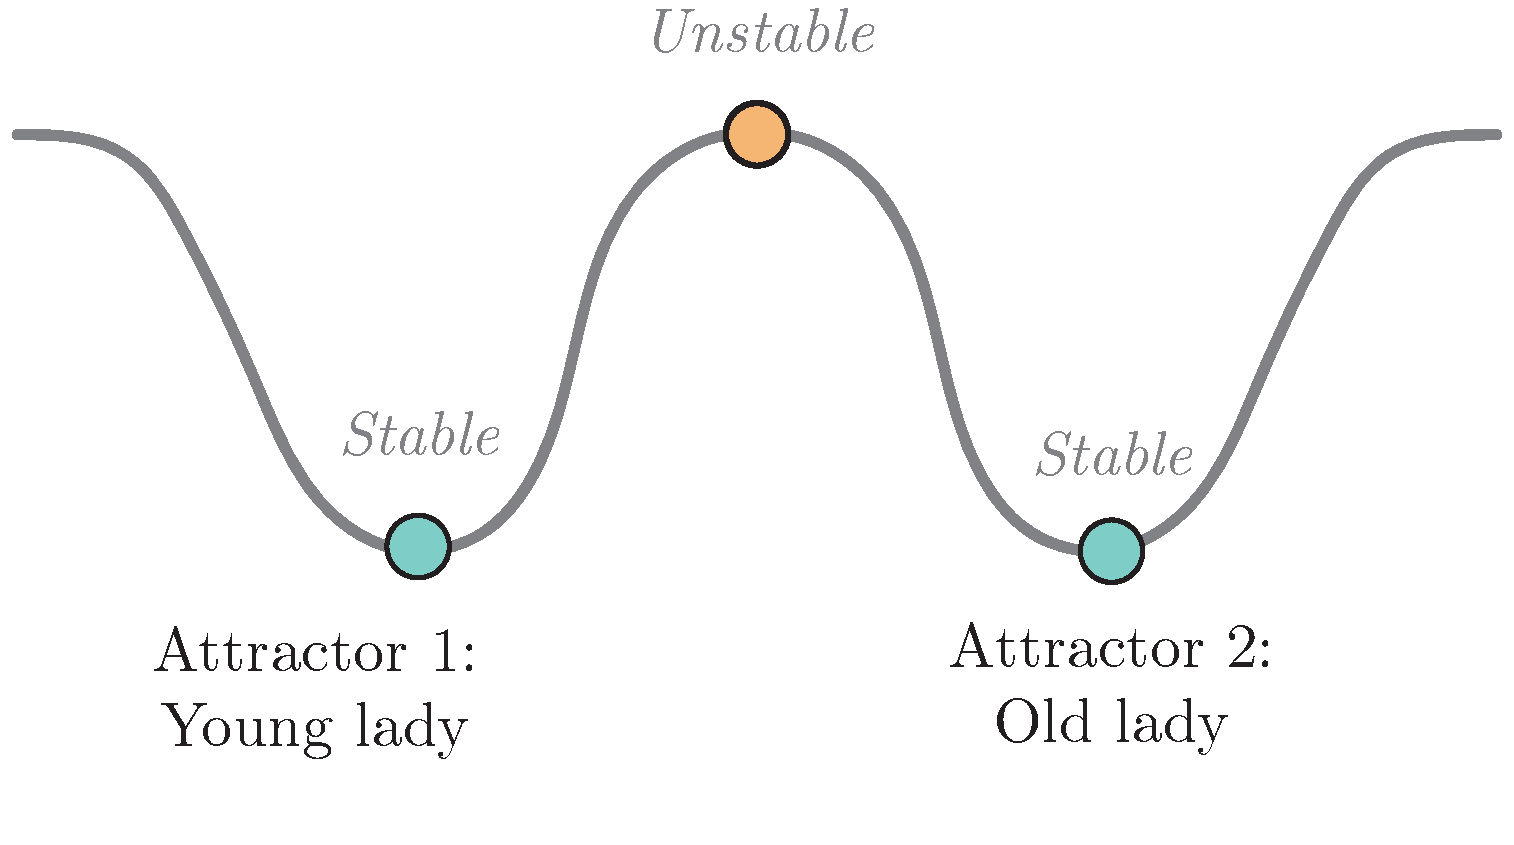
\includegraphics[width=.45\textwidth]{background/stability_plot_yougoldwoman.pdf} \\
(a) & (b)
\end{tabular}
\caption{(a) My Wife and My Mother-In-Law, by the cartoonist W. E. Hill, 1915 (b) Stability plots illustrating the two attractors of the cartoon as proposed by~\citet{dilts1995nlp}}
\label{fig:youngoldlady}
\end{figure}

As displayed in \fig{fig:example_self_org}, nature is full of examples of self-organizing systems. Physical systems exhibit self-organizing behavior through the formation of patterns, such as the longitudinal stripes of sand dunes or the crystalline structure of snowflakes. Similarly, biological systems display self-organizing behaviors\citep{camazine2001self-organization}, as exhibited in the social organization of fish schools and insect swarms, as well as in their ability to collectively adapt to and modify their environment when termites construct mounds and bees build their hives.
%
\begin{figure}[!h]
\small
\centering
\begin{tabular}{c}
	(a) Physical self-organizing systems\\
	
\includegraphics[width=.6\textwidth]{background/self_organizing_physical.pdf}\\
	(b)Biological self-organizing systems\\
	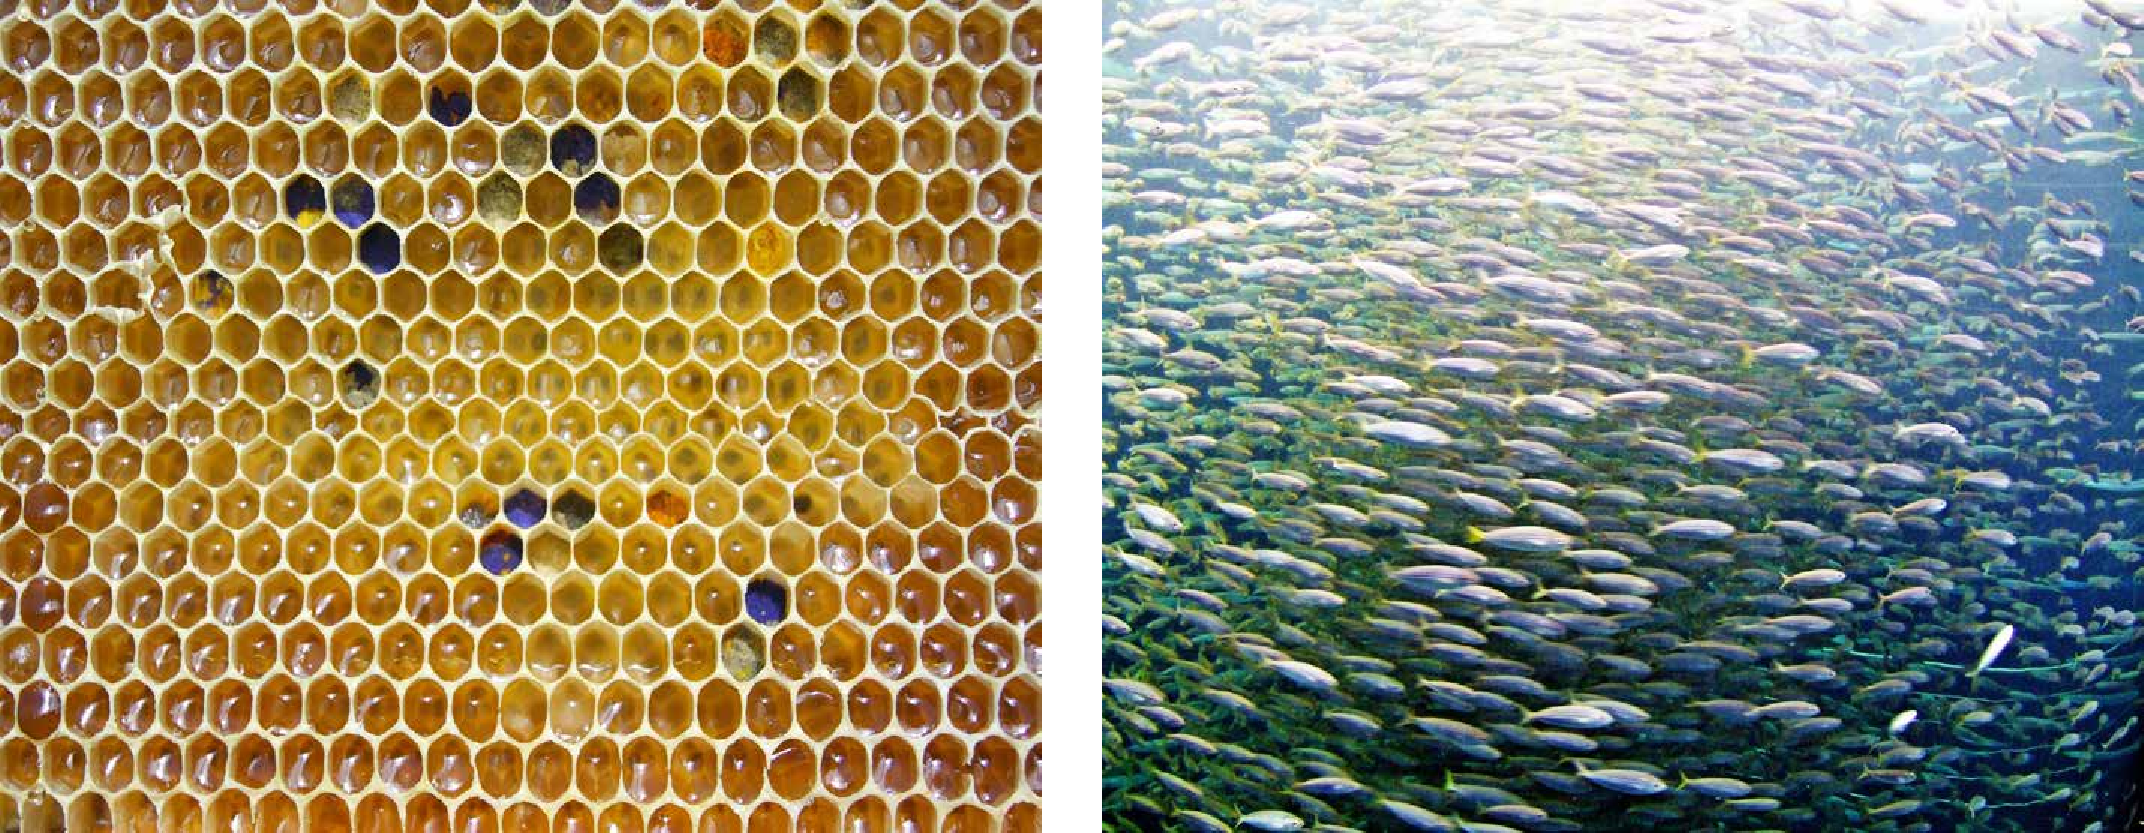
\includegraphics[width=.6\textwidth]{background/self_organizing_biological.pdf}
\end{tabular}
\caption{Example of self-organizing systems (a) sand dunes in Namibia and crystal structure of snow ice; and (b) a bee comp and a fish school. Images are royalty-free and obtained from \url{pixabay.com}}
\label{fig:example_self_org}	
\end{figure}

Self-organization also enables creative technical innovation such as the development of self-organizing traffic lights~\citep{ferreira2010self-organized}: lights that can adapt to changing traffic conditions through local interactions, rather than relying on communication or external signals. Self-organization is particularly well suited for the problem of traffic light regulation because traffic conditions change constantly. Thus, the problem at hand is not one of optimization, but rather of adaptation, and self-organization seems to be better equipped to handle this type of challenge.

\paragraph{Self-organization in Developmental \ai}

Developmental \ai problems can be formulated as adaptive problems where one or more agents and the environment are coupled dynamical systems whose interactions are responsible for the agents' behavior~\citep{beer1995dynamical}. In this research, we propose to use the language of dynamical systems and the theory of self-organization to formalize the two fundamental problems of this research.

 First, the problem of the emergence of cultural convention among artificial agents can be analyzed as the self-organization of a language community~\citep{steels1995selforganizing,oudeyer2005selforganization}. A cultural convention is thus an attractor of a language community: when multiple agents interact, variations of language behaviors are attracted to an equilibrium state because the more members of a community adopt a particular convention, the stronger the convention becomes. We will present several approaches that model language acquisition in \sect{sec:self-orga-lang}. 

Second, the problem of autonomous skill acquisition can be framed as the self-organization of agents' trajectories where agents use internal mechanisms to develop rather than being controlled by hierarchical top-down control~\citep{pfeifer2007robotics}. In this context, agents develop and grow repertoires of skills via internal drivers. These internal drivers, referred to as intrinsic motivations~\citep{oudeyer2005selforganization}, allow agents to self-organize their behavior into developmental trajectories and enable them to acquire increasingly complex skills. We will explore the open-ended skill acquisition problem and present various approaches to it in \sect{sec:self-orga-traj}.

In order to tackle the two challenges outlined previously, this study builds upon the standard \ai techniques presented in \sect{sec:standard_ai}. However, it should be noted that these two challenges cannot be simply reduced to optimizing a single objective. The aim of this research is not solely to produce specific behaviors, but rather to understand the key cognitive mechanisms that can explain their emergence. As such, when examining communication among agents, our analysis will encompass not only the agents' communicative capabilities but also the structure of the language that emerges. Similarly, when evaluating the abilities of autonomous agents, our assessment will include not only their skill performance, but also their exploration strategies and trajectories. These considerations are further discussed in the following two sections, which both include a paragraph dedicated to evaluating emergent phenomena.

\newpage
\subsection{Self-organisation of Cultural Convention and the Language Acquisition Problem}
\label{sec:self-orga-lang}

The study of the origin of language has been a subject of interest and debate among various academic disciplines, including linguistics, archaeology, biology, and anthropology. In this section, we will shortly present the predominant theories on language acquisition and explore how artificial agents can help experiment with them. For a thorough review of the synthetic modeling of language origins see \citet{steels1997evolution}. There are three predominant theories on the origin of language:
\begin{enumerate}[noitemsep]
\item The \textit{Genetic evolution theory} postulates that language, just like biological complexity,  is the result of natural selection. According to this theory, humans have an innate language organ inside their brains that contains universal rules helping them learn a language during their development. This claim is backed by the famous poverty of stimulus argument which asserts that children do not observe sufficient data to explain their ability to acquire natural language~\citep{chomsky1975reflections}. The genetic evolution theory thus implies that there exist language genes that code for the language organ and that language is preserved due to genetic transmission. 
\item The \textit{Adaptation and self-organization theory} on the other hand supposes that language is preserved in the memories of individuals and transmitted through cultural and social interactions during imitation and acquisition processes. In the adaptation hypothesis, there is no language organ but rather a variety of cognitive and motor primitives that facilitate language acquisition. 
\item The \textit{Genetic assimilation theory} assumes that language is the result of dual dynamics that both involve cultural and genetic interactions. The genetic assimilation hypothesis is also known as the Baldwin effect. It states that learned behaviors that confer a selective advantage can become genetically encoded over time.  The genetic assimilation theory proposes that initially, humans did not have an innate language structure and that the first forms of language were acquired through adaptation only. But, if the speed of language acquisition played a role in selection, genetic assimilation would have facilitated the development of language acquisition devices.
\end{enumerate}

\paragraph{Language Acquisition with Artificial Agents}

The study of language emergence can benefit greatly from the utilization of agent-based modeling and simulation~\citep{Hurford1989BiologicalEO,birghton2002compositional,cangelosi2002simulating,steels2015talkingheads,kirby2014iterated}. \textit{Computational Experimental Semiotics}~\citep{galantucci2011experimental} is a field that analyzes the numerous factors that contribute to language emergence by examining a population of simulated agents engaging in two distinct types of interaction: \textit{linguistic} and \textit{genetic interactions}. When two agents take part in linguistic interaction, they are in turn speakers and listeners and respectively produce and receive messages describing a context. To study the formation of meanings, linguistic interactions occur within physical environments that contain objects and embodied situations~\citep{steels2012grounded}. Depending on the communicative success of linguistic interactions, agents can update their internal state and adapt to their artificial peers. To investigate the impact of population dynamics, the studied population is open: new agents enter, and others leave. These new agents, generated through genetic interactions and subject to potential mutations, introduce an element of novelty into the system. Finally, in order to obtain realistic models, the population should be studied as a distributed multi-agent system, i.e. there should not be any main global agent that acts over the entire population. Moreover, just like humans cannot enter the brain of others, agents should not be able to access each other's internal states.  A diagram of interactions as well as a high-level algorithmic implementation of the language acquisition framework is provided in \fig{fig:language_acquisition_framework} and Alg.~\ref{alg:langage-acquisition}.
\begin{figure}[!h]
\centering
\vspace{-.5cm}
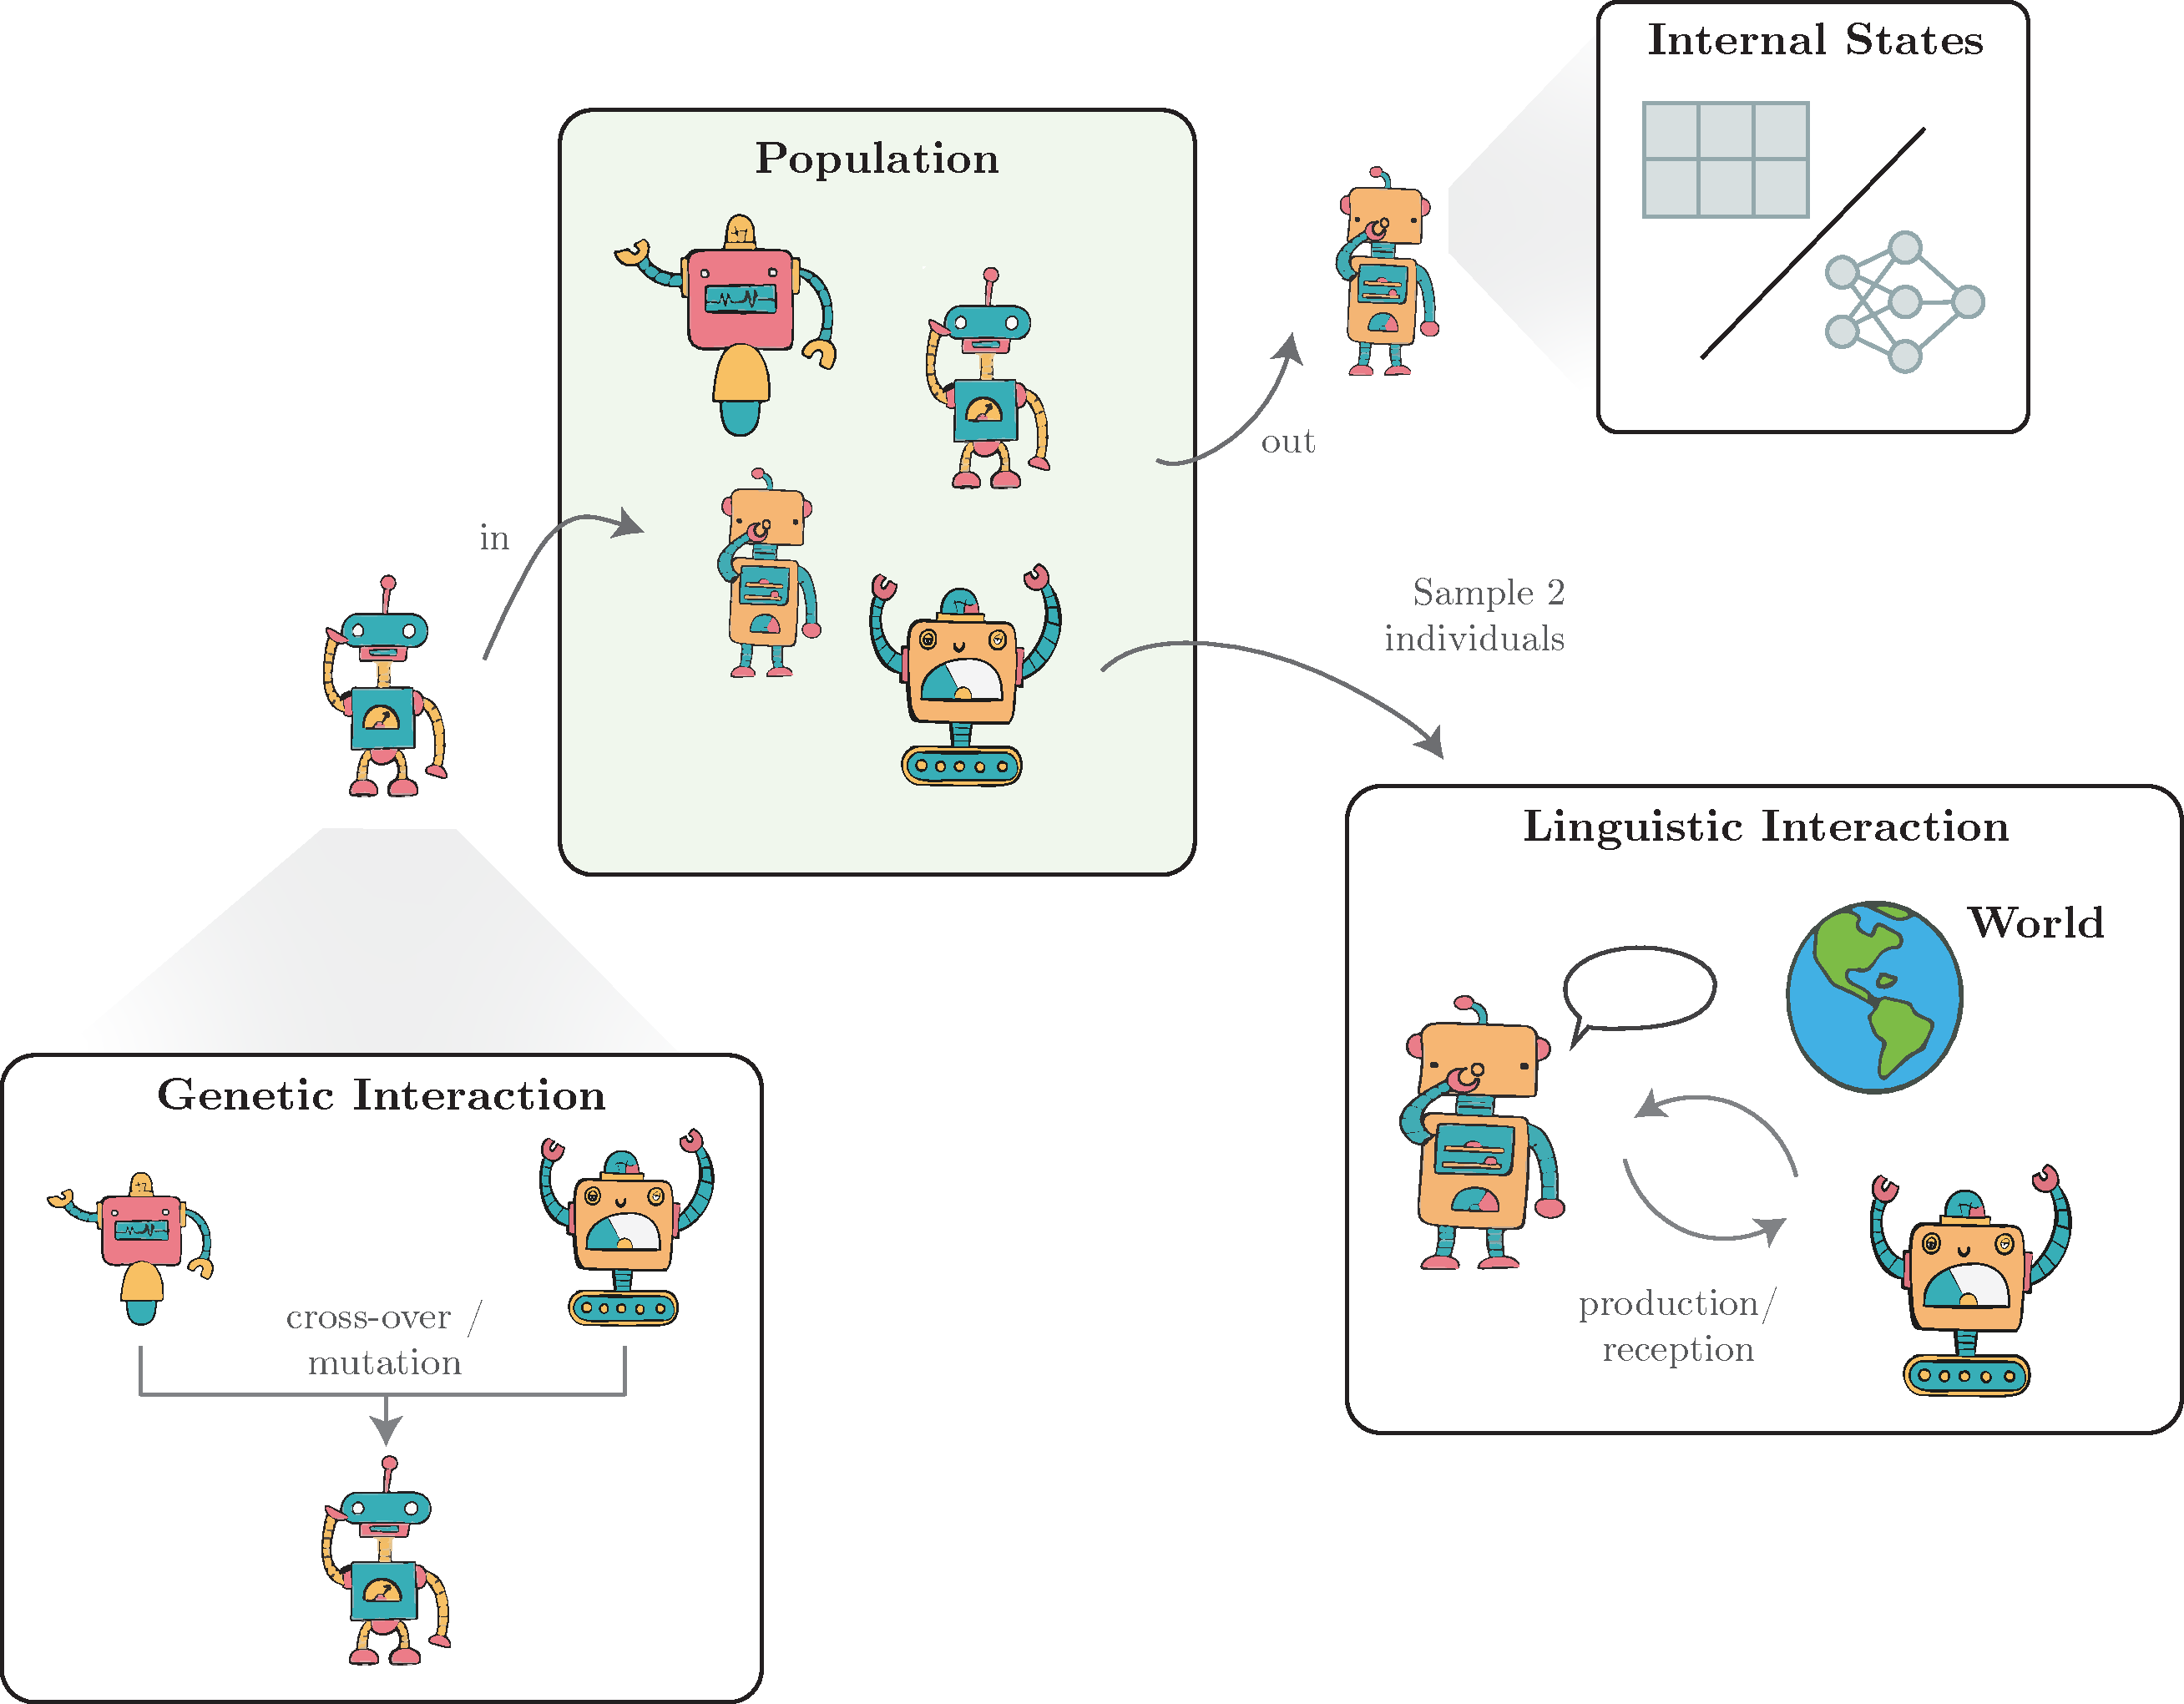
\includegraphics[width=.85\textwidth]{background/language_acquisition_framework.pdf}	
\caption{The language acquisition framework: A population of agents is an open multi-agent system where new agent enters and others leave. New agents are generated by genetic interactions: crossovers between parents with potential mutations. Agents have internal states allowing them to map signals to actions. They can perform linguistic interactions, i.e. exchanging messages to describe a physical situation of the world.}
\label{fig:language_acquisition_framework}
\end{figure}
%
\begin{algorithm}[!h]
    \begin{algorithmic}
    \small
        \caption{\label{alg:langage-acquisition}Language Acquisition Simulation}
        \REQUIRE Language Interaction $L$, Genetic Interaction $G$, Environment $\mathcal{E}$
        \STATE \textbf{Initialize} Population $\mathcal{P}_A$ and internal states of agents 
		\LOOP
        \STATE Sample two agents from population: $(A_1,A_2) \sim \mathcal{P}_A$ 
        \STATE Store result of linguistic interaction about the world: $ \leftarrow L(A_1,A_2,\mathcal{E})$
        \STATE Update $A_1$ and $A_2$ based on score $s$
        \STATE \textbf{With prob $p_{\text{out}}$:}
        \bindent
        \STATE Remove agent from population: $\mathcal{P}_A$.pop()
        \eindent
        \STATE \textbf{With prob $p_{\text{in}}$:}
        \bindent
        \STATE Sample two parents from population: $(A_1,A_2) \sim \mathcal{P}_A$  
        \STATE Perform Genetic Interaction: $A' \leftarrow G(A_1,A_2)$
        \STATE Add child to population: $\mathcal{P}_A$.add($A'$)
        \eindent
        \ENDLOOP
    \end{algorithmic}
\end{algorithm}

This study will not investigate the impact of population dynamics on the emergence of language. Rather, it will focus on the development of agents during a lifetime and disregard any genetic interactions. We will thus focus on the self-organization of cultural conventions during linguistic interactions. We will restrict our analysis to the smallest population of two individuals. 

\newpage
\paragraph{Language Games}

The simplest forms of linguistic interaction are coined language games. They derive from \textit{Signaling Games} introduced by \citet{Lewis1969} as a game theoretic approach to the problem of the emergence of conventions. In game theoretic words, a convention is a system of arbitrary rules that enables two players to share meaningful information.  \fig{fig:lewis_game} presents a simple example of a Lewis game. The two players of a signaling game are the speaker and the listener. In our example, the world is providing two world states to the speaker ($w_1$ and $w_2$). Based on the world state, the speaker sends a signal to the listener. Here, there are two available signals ($s_1$ and $s_2$). From the received signal, the listener then chose an action (among two actions $a_1$ and $a_2$). If the listener picks the correct action for the associated word state then both agents perceive a reward. Note that the Listener never perceives the world state.  
\begin{figure}[!h]
\centering
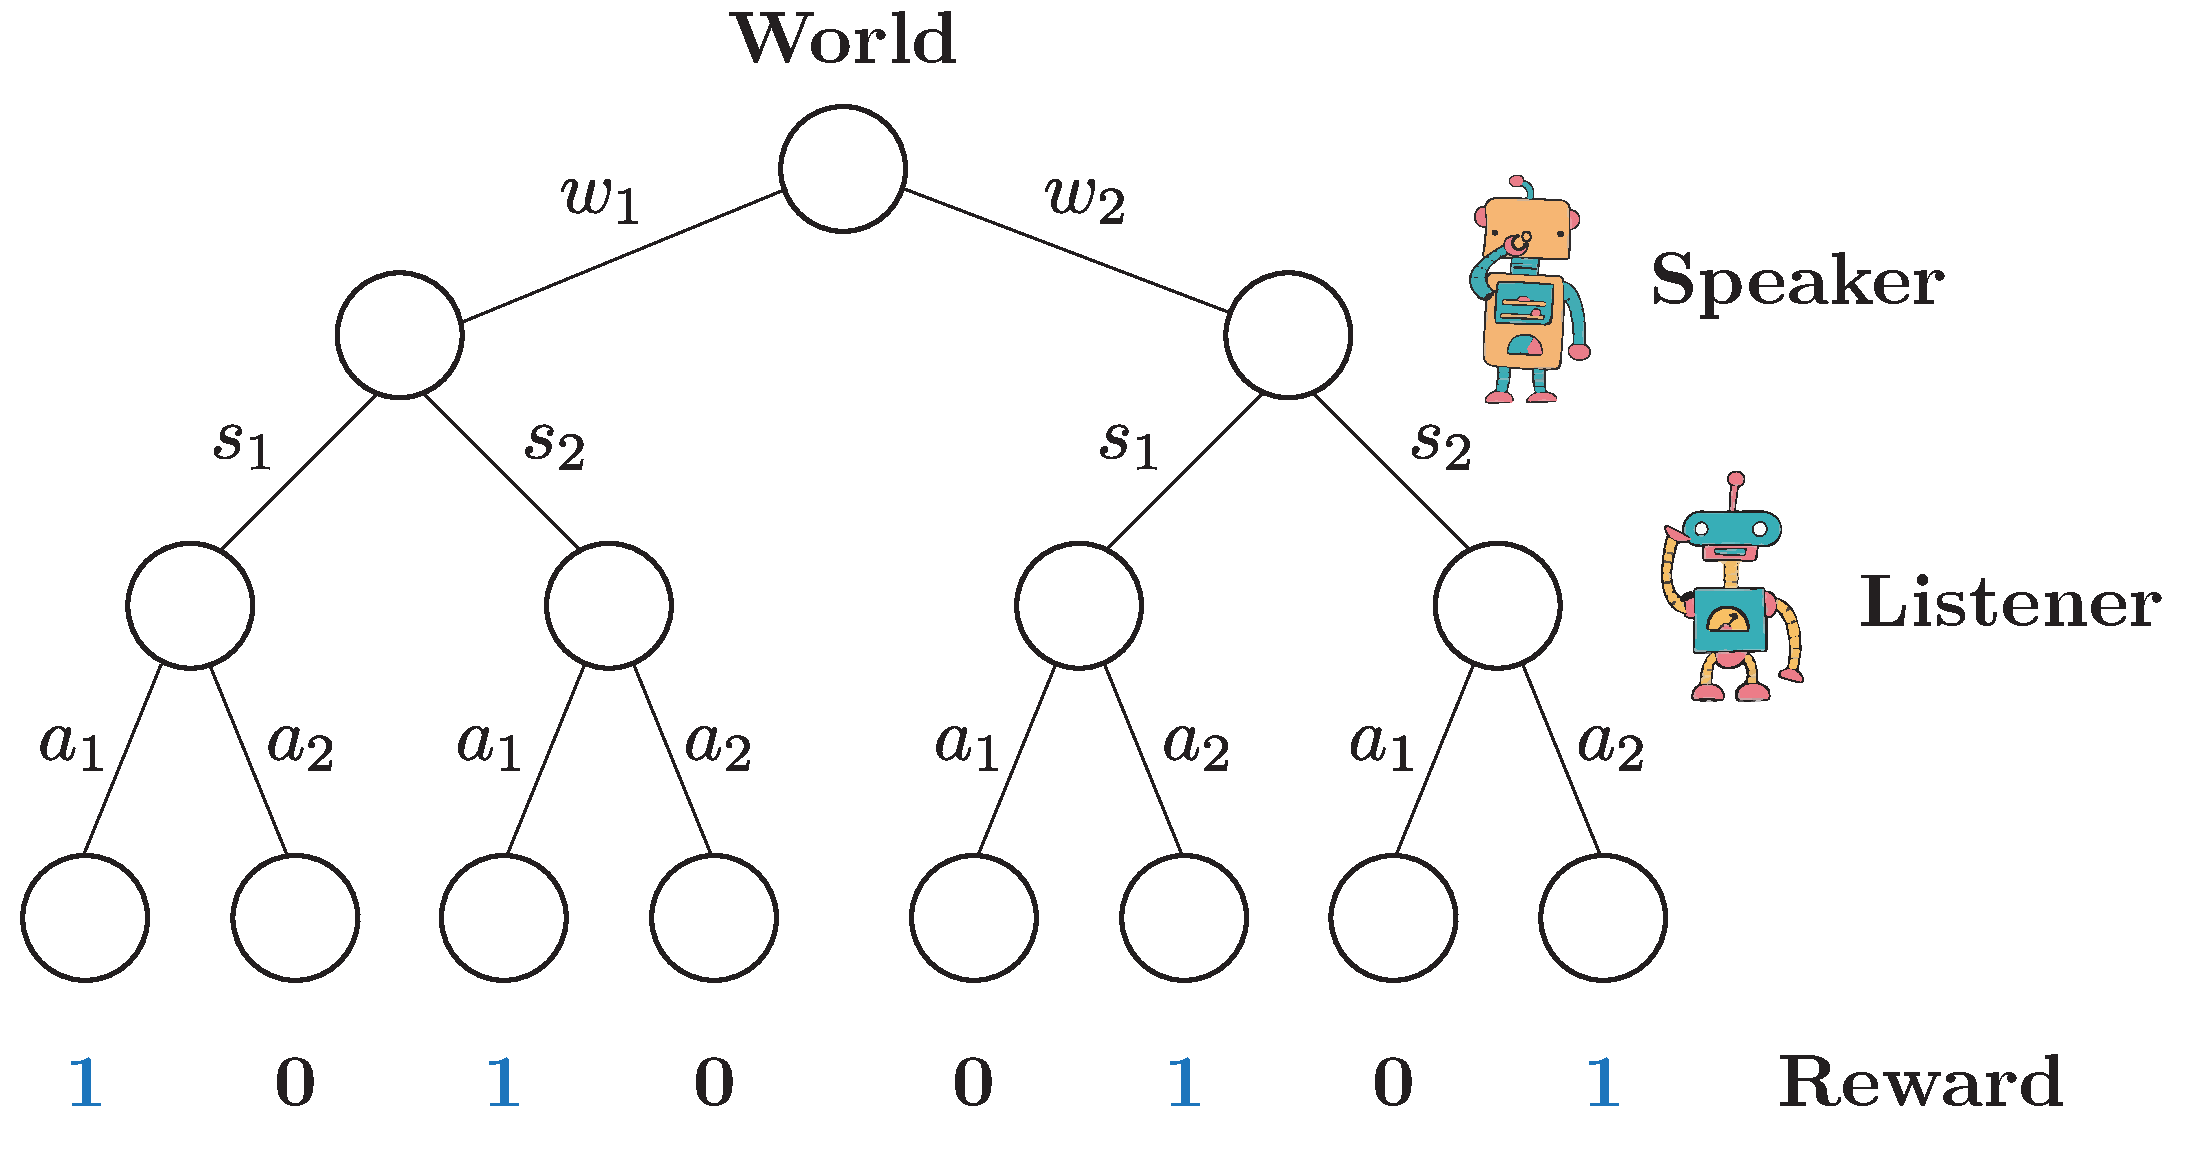
\includegraphics[width=.525\textwidth]{background/lewis_game.pdf}
\caption{Illustration of Lewis Signalling game with two world states, two signs, and two actions.}
\label{fig:lewis_game}
\end{figure}

To investigate the self-organization of conventions around meanings in a more realistic scenario, \citet{steels2012grounded} proposed to update signaling games with grounding elements.  In a grounded language game, the speaker and the listener are given a shared \textit{context} made of several \textit{referents} (objects) as displayed in \fig{fig:language_game_interactions}. The speaker samples a target referent from the context and produces an utterance to name it. Then, the speaker receives the utterance and picks a referent inside the context. If the chosen referent matches the target referent, the game is a success. To self-organize a language, a population of artificial agents needs to play numerous language games. In doing so, agents will alternate between speakers and listers. Depending on the outcome of the game they will update their internal states to reinforce successful conventions and diminish unsuccessful ones. Note that several update strategies are possible. They vary in how the outcome is actually perceived by the agents. On the speaker side, the referent ground truth (target) is known so the outcome of the game can be directly used for the update. On the other hand, since the listener does not know about the target referent some implementations of language games do not communicate the outcome to the listener. In \citet{steels2001language}'s formulation of language game, the outcome is communicated to the speaker via a retroactive pointing mechanism. The speaker basically points toward the target referent at the end of the game to communicate the outcome to the speaker.

\begin{figure}[!h]
\centering
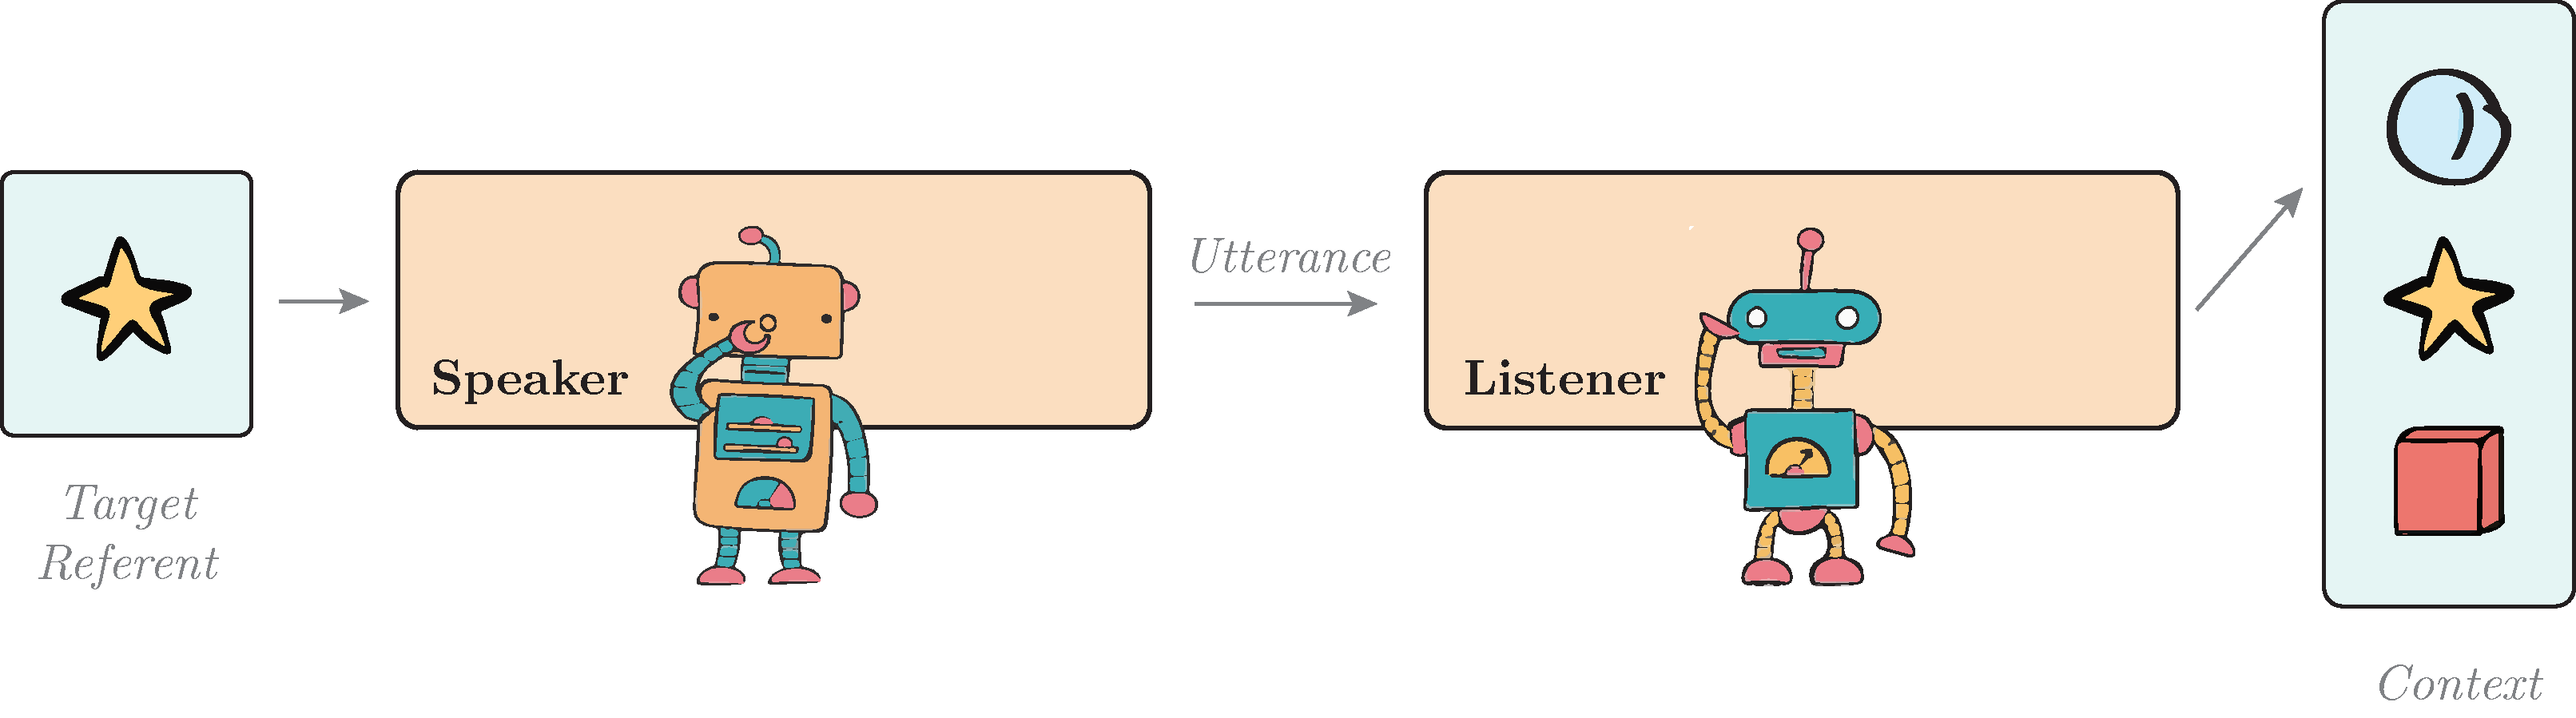
\includegraphics[width=.8\textwidth]{background/language_game_interactions.pdf}	
\caption{Diagram of interactions in a language game}
\label{fig:language_game_interactions}
\end{figure}

Early solutions to the language game~\citep{lipowska2011naming,steels2012grounded} use tables scoring associations between referents and utterances. Given fixed predefined numbers of utterances and referent categories, the agents can adjust the score of utterance/referent association depending on their communicative success. Examples of such tables for the speaker (left) and for the listener (right) are given in \fig{fig:language_game_tabular}.  If predefined referent categories are not available to the agents, \citet{steels2012grounded} propose mechanisms to map visual inputs to object categories. Similarly, the Talking Head experiments~\citep{steels2015talkingheads} propose strategies to adapt the language game to more realistic configurations with flexible and dynamic inventories of words and meanings.

\begin{figure}[!h]
\centering
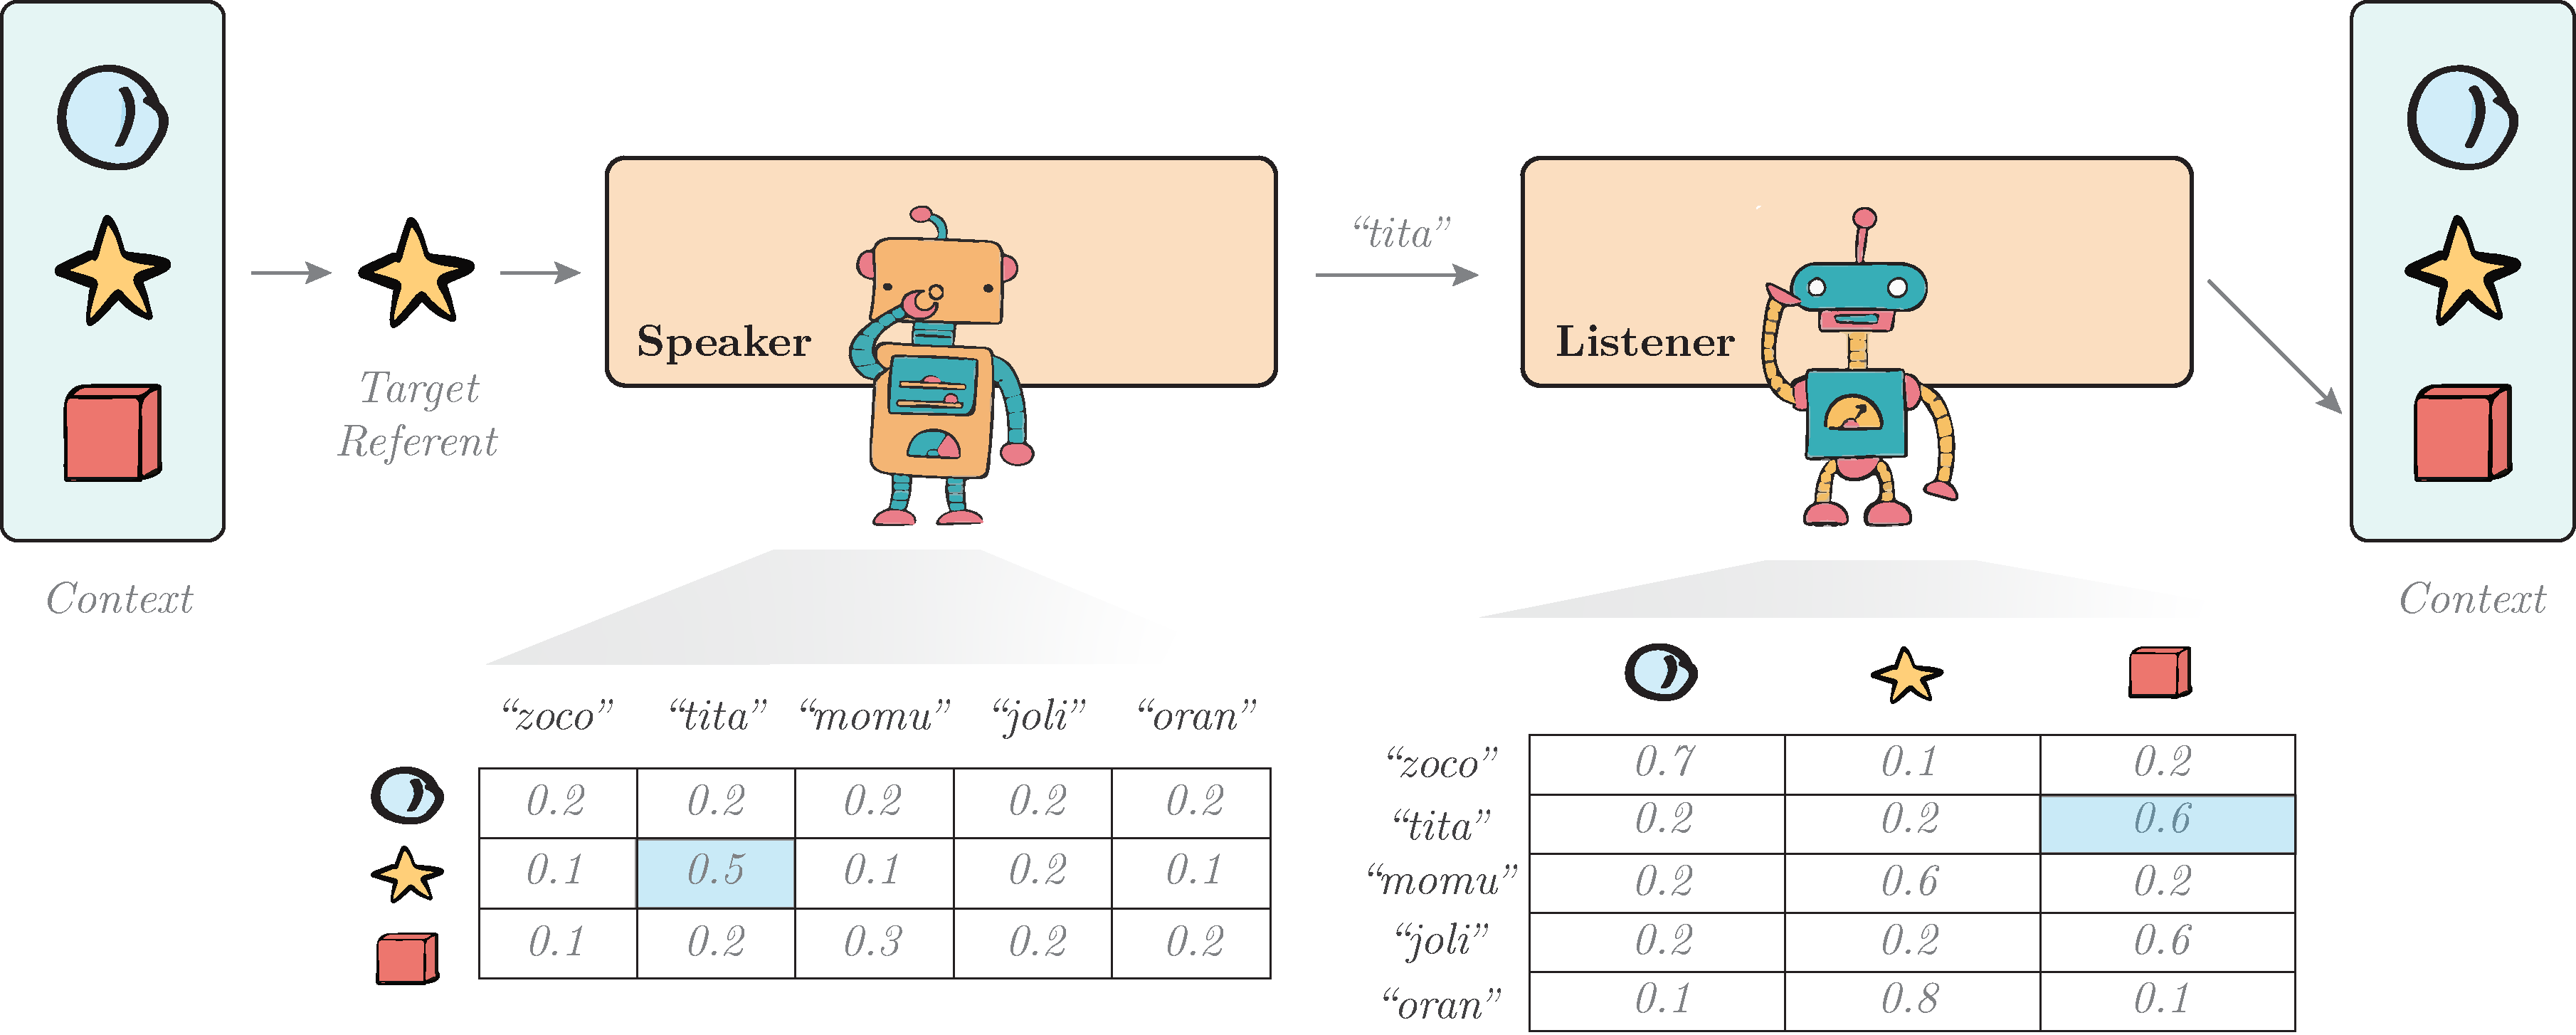
\includegraphics[width=.8\textwidth]{background/language_game_tabular.pdf}	
\caption{Example of agents' tabular internal models, with 3 referents and 5 words.}
\label{fig:language_game_tabular}
\end{figure}

\paragraph{Neural Communicating Agents}

Inspired by the success of Convolutional Neural Network in Computer Vision, \citet{lazaridou2017multiagent} proposed to extend language games to image referents with agents using neural networks to take actions \footnote{In deep learning, language games are often referred to as referential games or guessing games}. \fig{fig:language_game_network} illustrates their setup. The context is made of two images ($i_1$ and $i_2$), a target ($t$) and a distractor. The utterances are discrete utternaces $u$ coming from a fixed-sized dictionary $\mathcal{V}$.  The speaker's utterance is given by a neural network parametrizing a policy that maps the two images to the utterance: $u=\pi_S(i_1,i_2,t; \theta_S)$. Similarly, the listener uses policy $\pi_L$ to make a choice given the utterance: $a=\pi_L(i_1,i_2,\pi_S(i_1,i_2,t; \theta_S);\theta_L)$. The policies are trained using \rl (\sect{sec:background_rl}) with reward function $R$ returning 1 iff $\pi_L(i_1,i_2,\pi_S(i_1,i_2,t; \theta_S);\theta_L) := t$. Note that in their implementation the reward and thus the outcome of the game is communicated to both agents which is equivalent to Steel's pointing mechanism. 

\begin{figure}[!h]
\centering
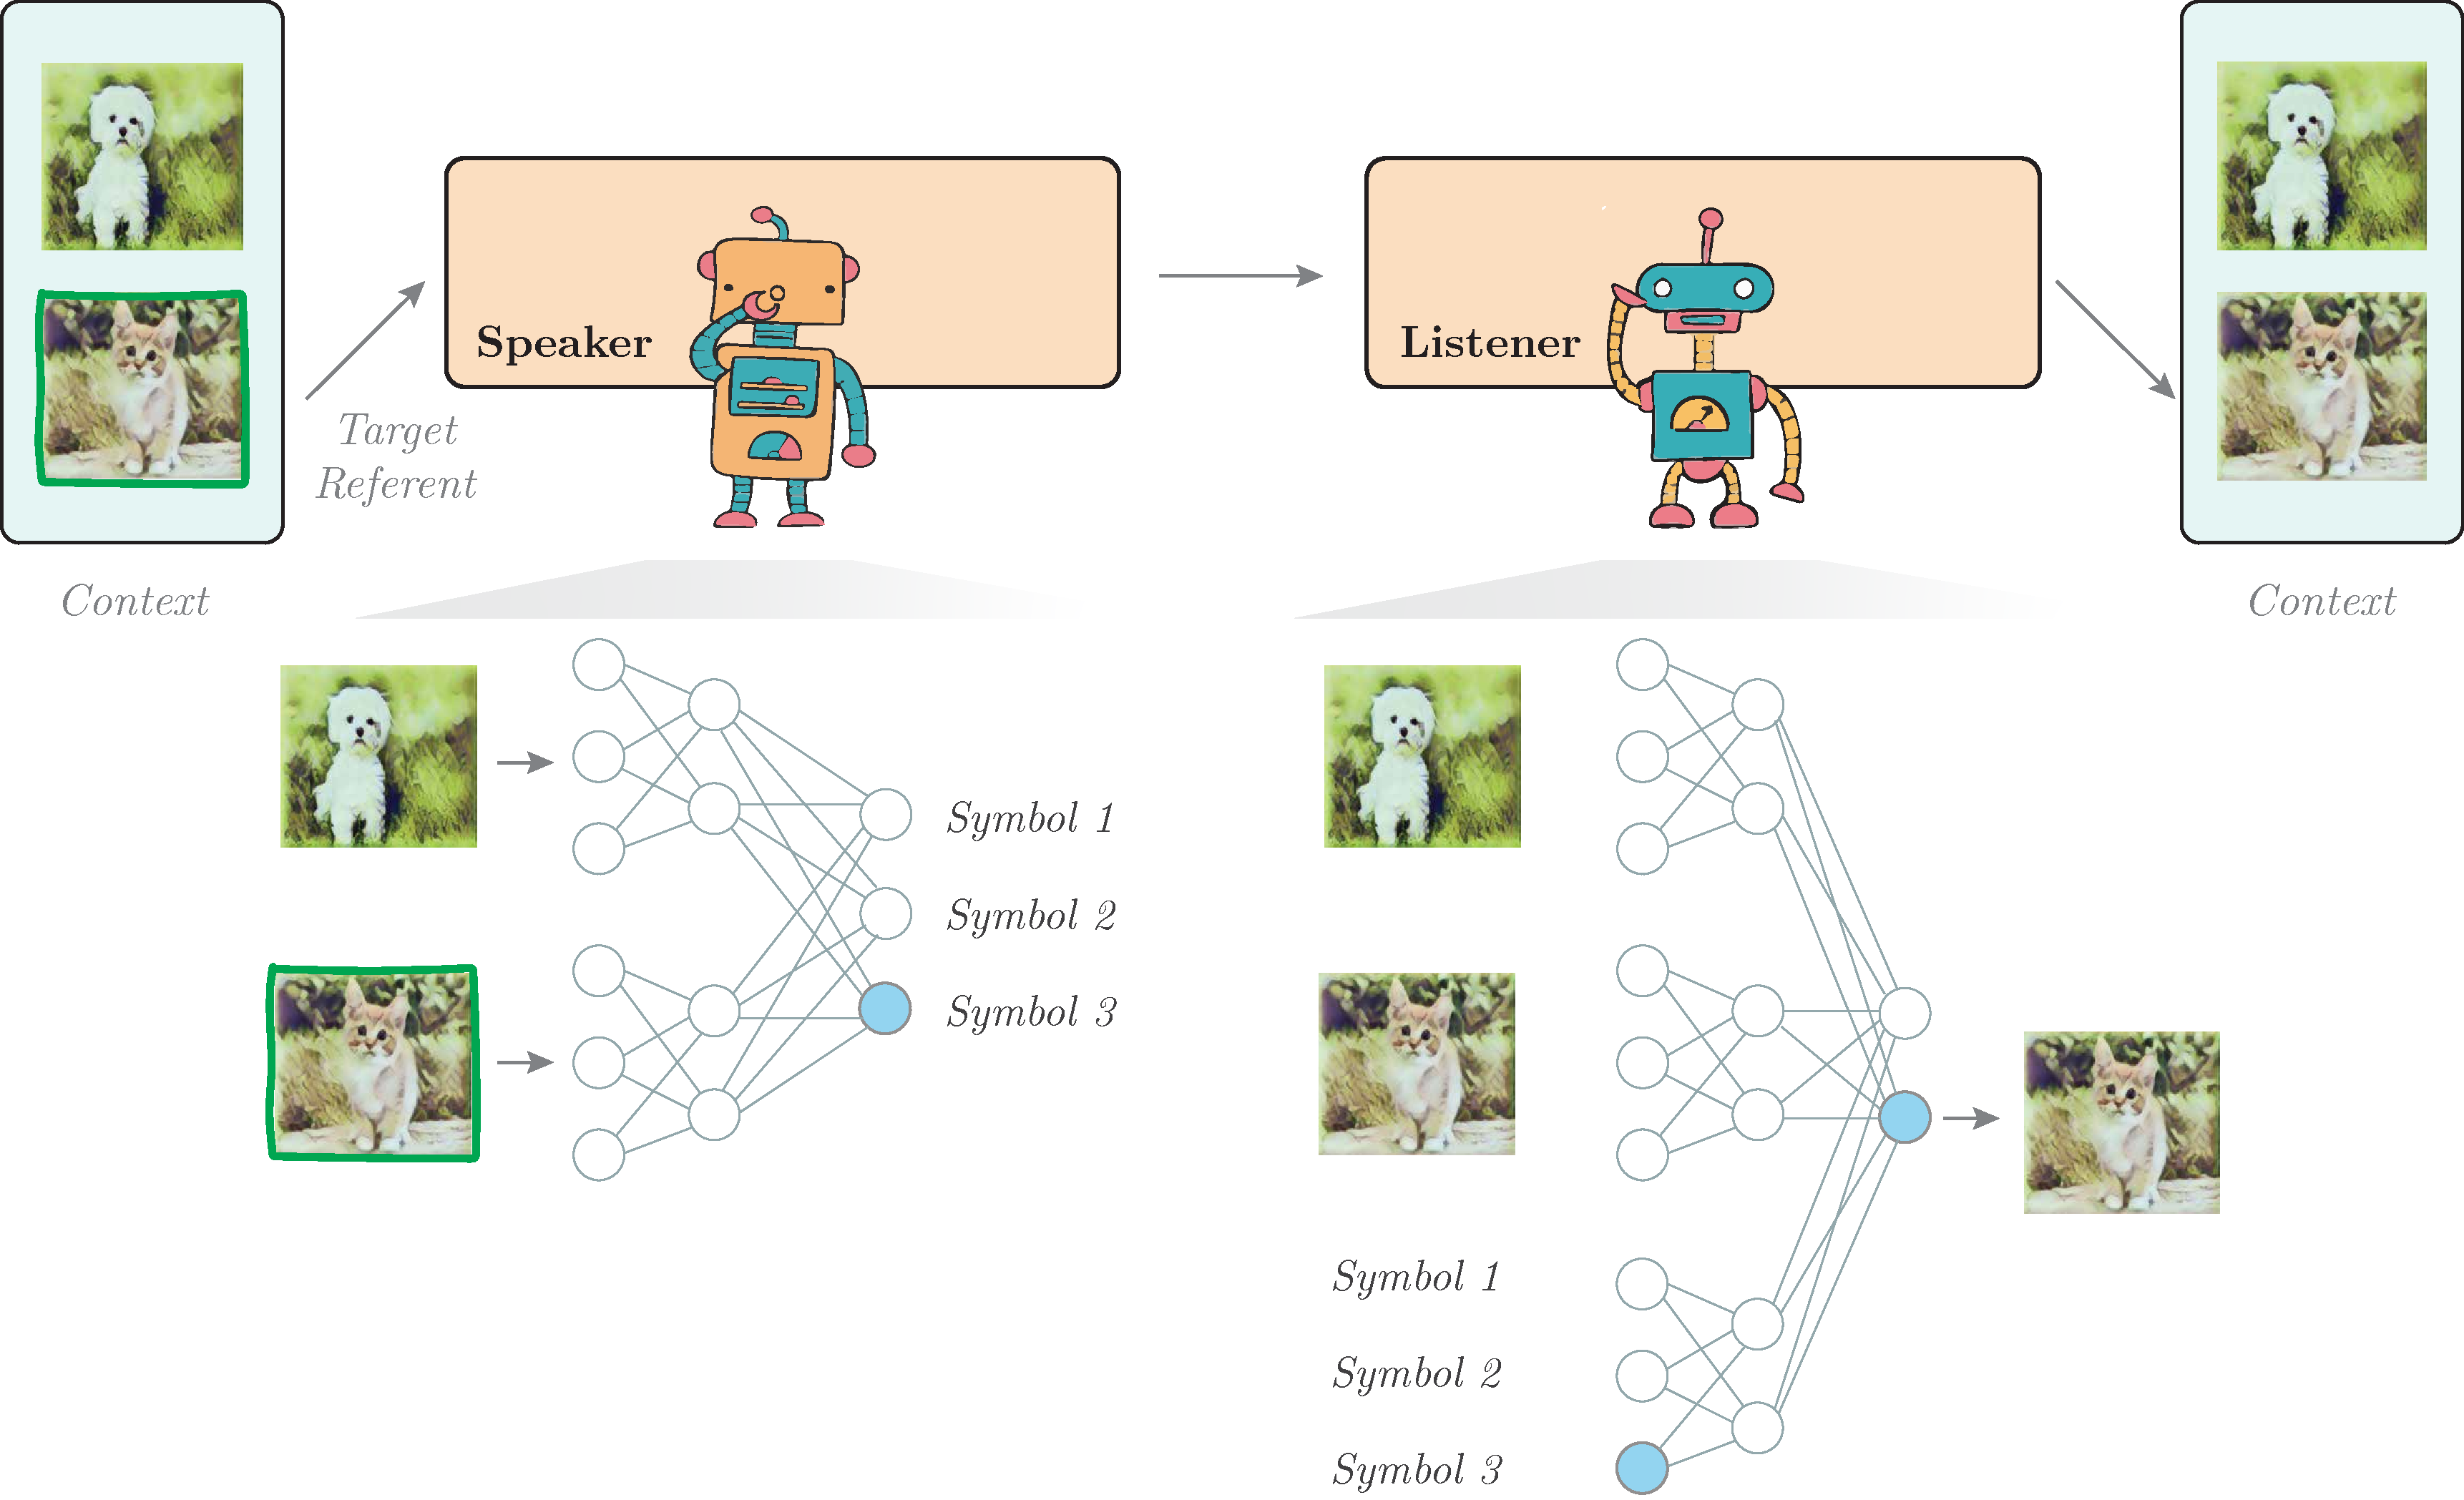
\includegraphics[width=.75\textwidth]{background/language_game_network.pdf}	
\caption{Example of agents' neural network internal models, with 2 referents and 3 words (adapted from \citet{lazaridou2017multiagent}).}
\label{fig:language_game_network}
\end{figure}

Beyond scaling previous language game approaches to visual referents, \citet{lazaridou2017multiagent} propose a strategy to achieve human interpretable code. They demonstrate that alternating between \rl in the classical language game and standard supervised learning for image classification leads to the effective grounding of agents' code in natural language. In a similar study, \citet{havrylov2017emergence} examine the emergence of communication with sequences of symbols and visual referents. They use \lstms within the speaker and listener architectures to support the encoding and decoding of discrete tokens arranged in fixed-size sequences. They also analyze the compositionality and variability of the emerging sequences in both tabular-rasa and natural language communication. 

The identification of the factors that contribute to the emergence of compositional communication code is a fundamental objective within the field of computational linguistics. To this end, the use of neural communicating agents in language games has emerged as a valuable experimental setting. \citet{kottur2017natural} propose to analyze how utterances consisting of sequences of symbols can name referents that are compositions of abstract attributes (represented as one-hot vectors). The decomposition of referents into pre-defined hardcoded attributes enables a more comprehensive and systematic analysis of the compositional properties of the evolving communication code. Building upon this work, \citet{chaabouni2020compositionality} emphasize the importance of separating the compositional generalization capabilities of agents and compositional properties of the emerging code. They have established that the former can be achieved independently of the latter. Other works look at the environmental and internal factors that favor the emergence of compositionality. For instance, \citet{rodriguez-luna-etal-2020-internal} show that auxiliary objectives incentivizing object consistency or least effort (the generation of short sequences) support the emergence of compositional code in language games. Similarly, \citet{mu2021emergent} demonstrate that agents solving a variation of the language games where referents are organized in sets of objects agree on a more interpretable and systematic communication code. Finally, \citet{Ren2020Compositional} proposed to study the emergence of compositional code in a more complete setting with a population of agents playing language games over several generations.

\paragraph{Goal-Directed Communicating agents}

The prior paragraph demonstrates that guessing interactions provide an effective experimental testbed to study language acquisition. But, as outlined in the introduction, human language serves a multitude of purposes beyond mere object guessing. Therefore, \ai researchers have aimed to examine the development of communication in more realistic scenarios, where agents must communicate to accomplish a collaborative task in complex environments that involve interactions with the physical world across multiple time steps. These problems are modeled using \marl as described in \sect{sec:background_marl}. The agents must concurrently learn to interact with the world and communicate with others by observing rewards related to their collaborative goal, provided by an expert. See \fig{fig:marl_comm_interactions} for a visual representation of these interactions. Seminal works on \marl involving communicating agents consider problems such as efficient car coordination at traffic junctions to avoid collision~\citep{sukhbaatar2016learning} or riddles where agents need to combine environmental inputs with information communicated over several time steps to succed~\citep{foerster2016learning}. In their work, \citet{foerster2016learning} introduce two approaches for learning to communicate in \marl: Differentiable Inter-Agent Learning (\textsc{dial}) and Reinforced Inter-Agent Learning (\textsc{rial}). \textsc{dial} is based on the centralized training and decentralized execution method and enables gradient to be exchanged between agents, thereby breaking the assumption of the language acquisition framework that agents should not be able to have access to each other's internal states. Conversely, in \textsc{rial}, messages are viewed as actions produced by a \rl algorithm where each agent treats others as a part of the environment, without the need to have access to other agents’ internal parameters or to back-propagate gradients. The \textsc{rial} algorithm now serves as a baseline for a variety of \marl communication investigations. \cite{jiang2018learning} extended it with an attention mechanism that enables agents to learn when communication is required to solve collaborative tasks.  Similarly, \citet{eccles2019biases} showed that adding positive signaling (messages must be different in different situations) and positive listening (actions must be different when messages are different) biases to agents via auxiliary losses yields an increase in communicative performance. For a complete survey of emergent communication in \marl setups, see \citet{zhu2022survey}.

\begin{figure}[!h]
\centering
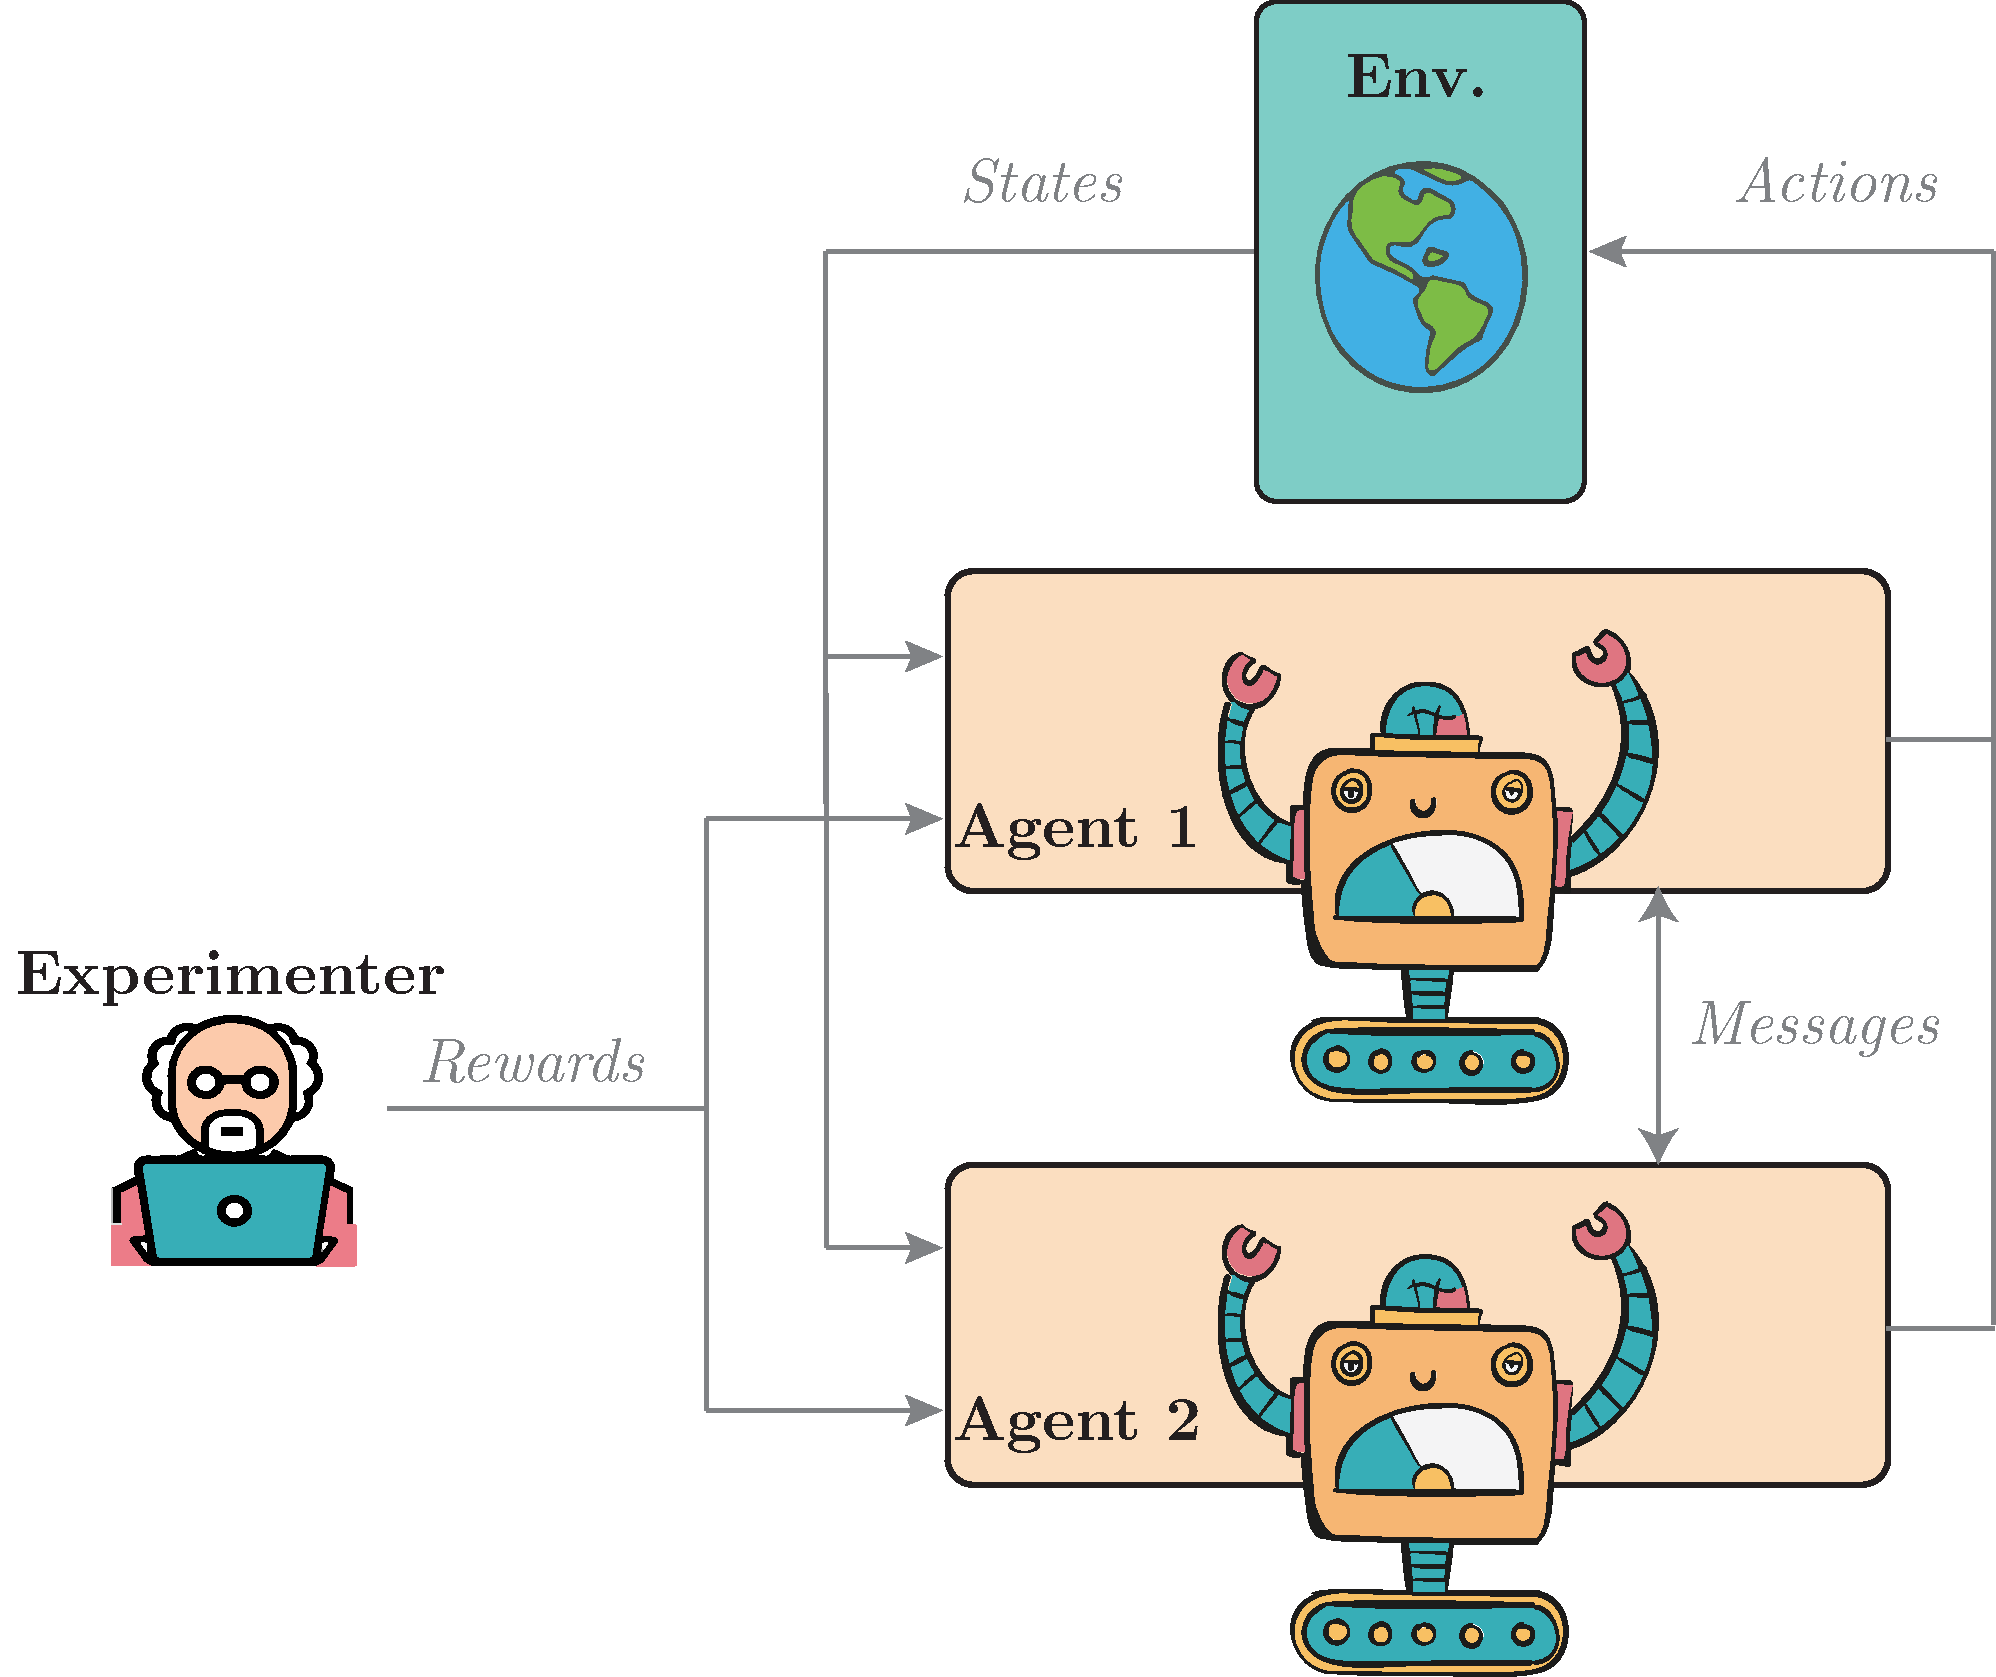
\includegraphics[width=.5\textwidth]{background/marl_comm_interactions.pdf}	
\caption{Diagram of interactions in \marl emergence communication setup.}
\label{fig:marl_comm_interactions}
\end{figure}


\paragraph{Conclusion and connection with our contributions}

In this section, we presented the language acquisition framework which study the emergence of communication inside a population of agents interacting within linguistic and genetic interactions. Our contributions focus on linguistic interactions and ignore the influence of population dynamics on the emergence of communication. We, therefore, presented the most broadly studied linguistic interactions: the language game. Additionally, we showed that this particular guessing interaction setup could be scaled to neural agents. Finally, we noted that \marl offers a valuable framework to study the emergence of communication as a tool to achieve collaborative behaviors in physically complex environments. Our first contribution (Chapter~\ref{chap:curves}) extends the language game framework to investigate the self-organization of a graphical communication code with visual referents and agents communicating via a sensory-motor channel. Our second contribution (Chapter~\ref{chap:abig}) investigates the emergence of communication in the scenario where agents have asymmetries of information and affordances, where the reward cannot be communicated to all agents.  

%
\newpage

\subsection{Self-organisation of Trajectories and the Open-ended Skill Acquisition Problem}
\label{sec:self-orga-traj}
%

Beyond modeling language acquisition, developmental \ai aims to model how children learn skills in general. In this study, we propose a computational framework that addresses the challenge of self-organizing developmental trajectories through intrinsically motivated skills acquisition. The framework, referred to as autotelic \rl, is a combination of developmental approaches and reinforcement learning (see the definition of autotelic in \sect{sec:humans_autotelic}).  It builds on \textit{intrinsic motivations} (\ims) to enable agents to learn to represent, generate, select, and solve their own problems. To provide a comprehensive understanding of the framework, we first present a typology of intrinsic motivation approaches in developmental \ai, followed by a presentation of the intrinsically motivated skills acquisition problem and its solution through autotelic reinforcement learning.


\paragraph{Intrinsic Motivations in Developmental AI}

 Developmental \ai aims to model children learning and, thus, takes inspiration from the mechanisms underlying autonomous behaviors in humans. Most of the time, humans are not motivated by external rewards but spontaneously explore their environment to discover and learn about what is around them. This behavior seems to be driven by \textit{intrinsic motivations} (\ims) a set of brain processes that motivate humans to explore for the mere purpose of experiencing novelty, surprise or learning progress~\citep{berlyne1966curiosity,gopnik1999scientist,kidd2015psychology,oudeyer2016evolution,gottlieb2018towards}. The integration of \ims into artificial agents thus seems to be a key step towards autonomous learning agents \citep{schmidhuber1991possibility,kaplan2007search}. In developmental robotics, this approach enabled sample efficient learning of high-dimensional motor skills in complex robotic systems \citep{santucci2020intrinsically}, including locomotion \citep{baranes2013active,martius2013information}, soft object manipulation \citep{rolf2013efficient,nguyen2014socially}, visual skills \citep{lonini2013robust} and nested tool use in real-world robots \citep{imgep}. Most of these approaches rely on \textit{population-based} optimization algorithms, non-parametric models trained on datasets of (policy, outcome) pairs. Population-based algorithms cannot leverage automatic differentiation on large computational clusters, often demonstrate limited generalization capabilities and cannot easily handle high-dimension perceptual spaces (\eg images) without hand-defined input pre-processing. For these reasons, developmental robotics could benefit from new advances in deep \rl.

These convergences can mostly be categorized in two ways depending on the type of intrinsic motivation (\ims) being used \citep{oudeyer2007intrinsic}:
\begin{itemize}
    \item
    \textbf{Knowledge-based IMs} are about prediction. They compare the situations experienced by the agent to its current knowledge and expectations, and reward it for experiencing dissonance (or resonance). This family includes \ims rewarding prediction errors \citep{schmidhuber1991possibility,pathak2017curiosity}, novelty \citep{bellemare2016unifying,burda2018exploration,raileanu2020ride}, surprise \citep{achiam2017surprise}, negative surprise \citep{berseth2019smirl}, learning progress \citep{lopes2012exploration,kim2020active} or information gains \citep{houthooft2016vime}, see a review in \citep{linke2019adapting}. This type of \im is often used as an auxiliary reward to organize the exploration of agents in environments characterized by sparse rewards. It can also be used to facilitate the construction of world models \citep{lopes2012exploration,kim2020active,sekar2020planning}.
    \item
    \textbf{Competence-based IMs}, on the other hand, are about control. They reward agents to solve self-generated problems, to achieve self-generated goals. In this category, agents need to represent, select and master self-generated goals. As a result, competence-based \ims were often used to organize the acquisition of repertoires of skills in task-agnostic environments \citep{baranes2010intrinsically,baranes2013active,santucci2016grail,forestier2016modular,nair2018visual,warde2018unsupervised,curious,blaes2019control,pong2019skew,imagine}. Just like knowledge-based \ims, competence-based \ims organize the exploration of the world and, thus, might be used to train world models \citep{baranes2013active,chitnis2020glib} or facilitate learning in sparse reward settings \citep{geppg}. We propose to use the adjective \textbf{autotelic}, from the Greek \textit{auto} (self) and \textit{telos} (end, goal), to characterize agents that are intrinsically motivated to represent, generate, pursue and master their own goals (\ie that are both intrinsically motivated and goal-conditioned).
\end{itemize}

\rl algorithms using \textit{knowledge-based} \ims leverage ideas from developmental robotics to solve standard \rl problems. On the other hand, \rl algorithms using competence-based \ims organize exploration around self-generated goals and can be seen as targeting a developmental robotics problem: the \textit{open-ended and self-supervised acquisition of repertoires of diverse skills}. 
 
\textit{Intrinsically Motivated Goal Exploration Processes} (\imgep) is the family of autotelic algorithms that bake competence-based \ims into learning agents \citep{imgep}. \imgep agents generate and pursue their own goals as a way to explore their environment, discover possible interactions and build repertoires of skills. This framework emerged from the field of developmental robotics \citep{oudeyer2007intrinsic,baranes2009proximo,baranes2010intrinsically,rolf2010goal} and originally leveraged population-based learning algorithms (\popimgep) \citep{baranes2009r,baranes2013active,forestier2016modular,imgep}. 

Recently, goal-conditioned \rl agents were also endowed with the ability to generate and pursue their own goals and learn to achieve them via self-generated rewards. We call this new set of autotelic methods \rlimgeps. In contrast, one can refer to externally-motivated goal-conditioned \rl agents as \rlemgeps.

\begin{figure}[!h]
\centering
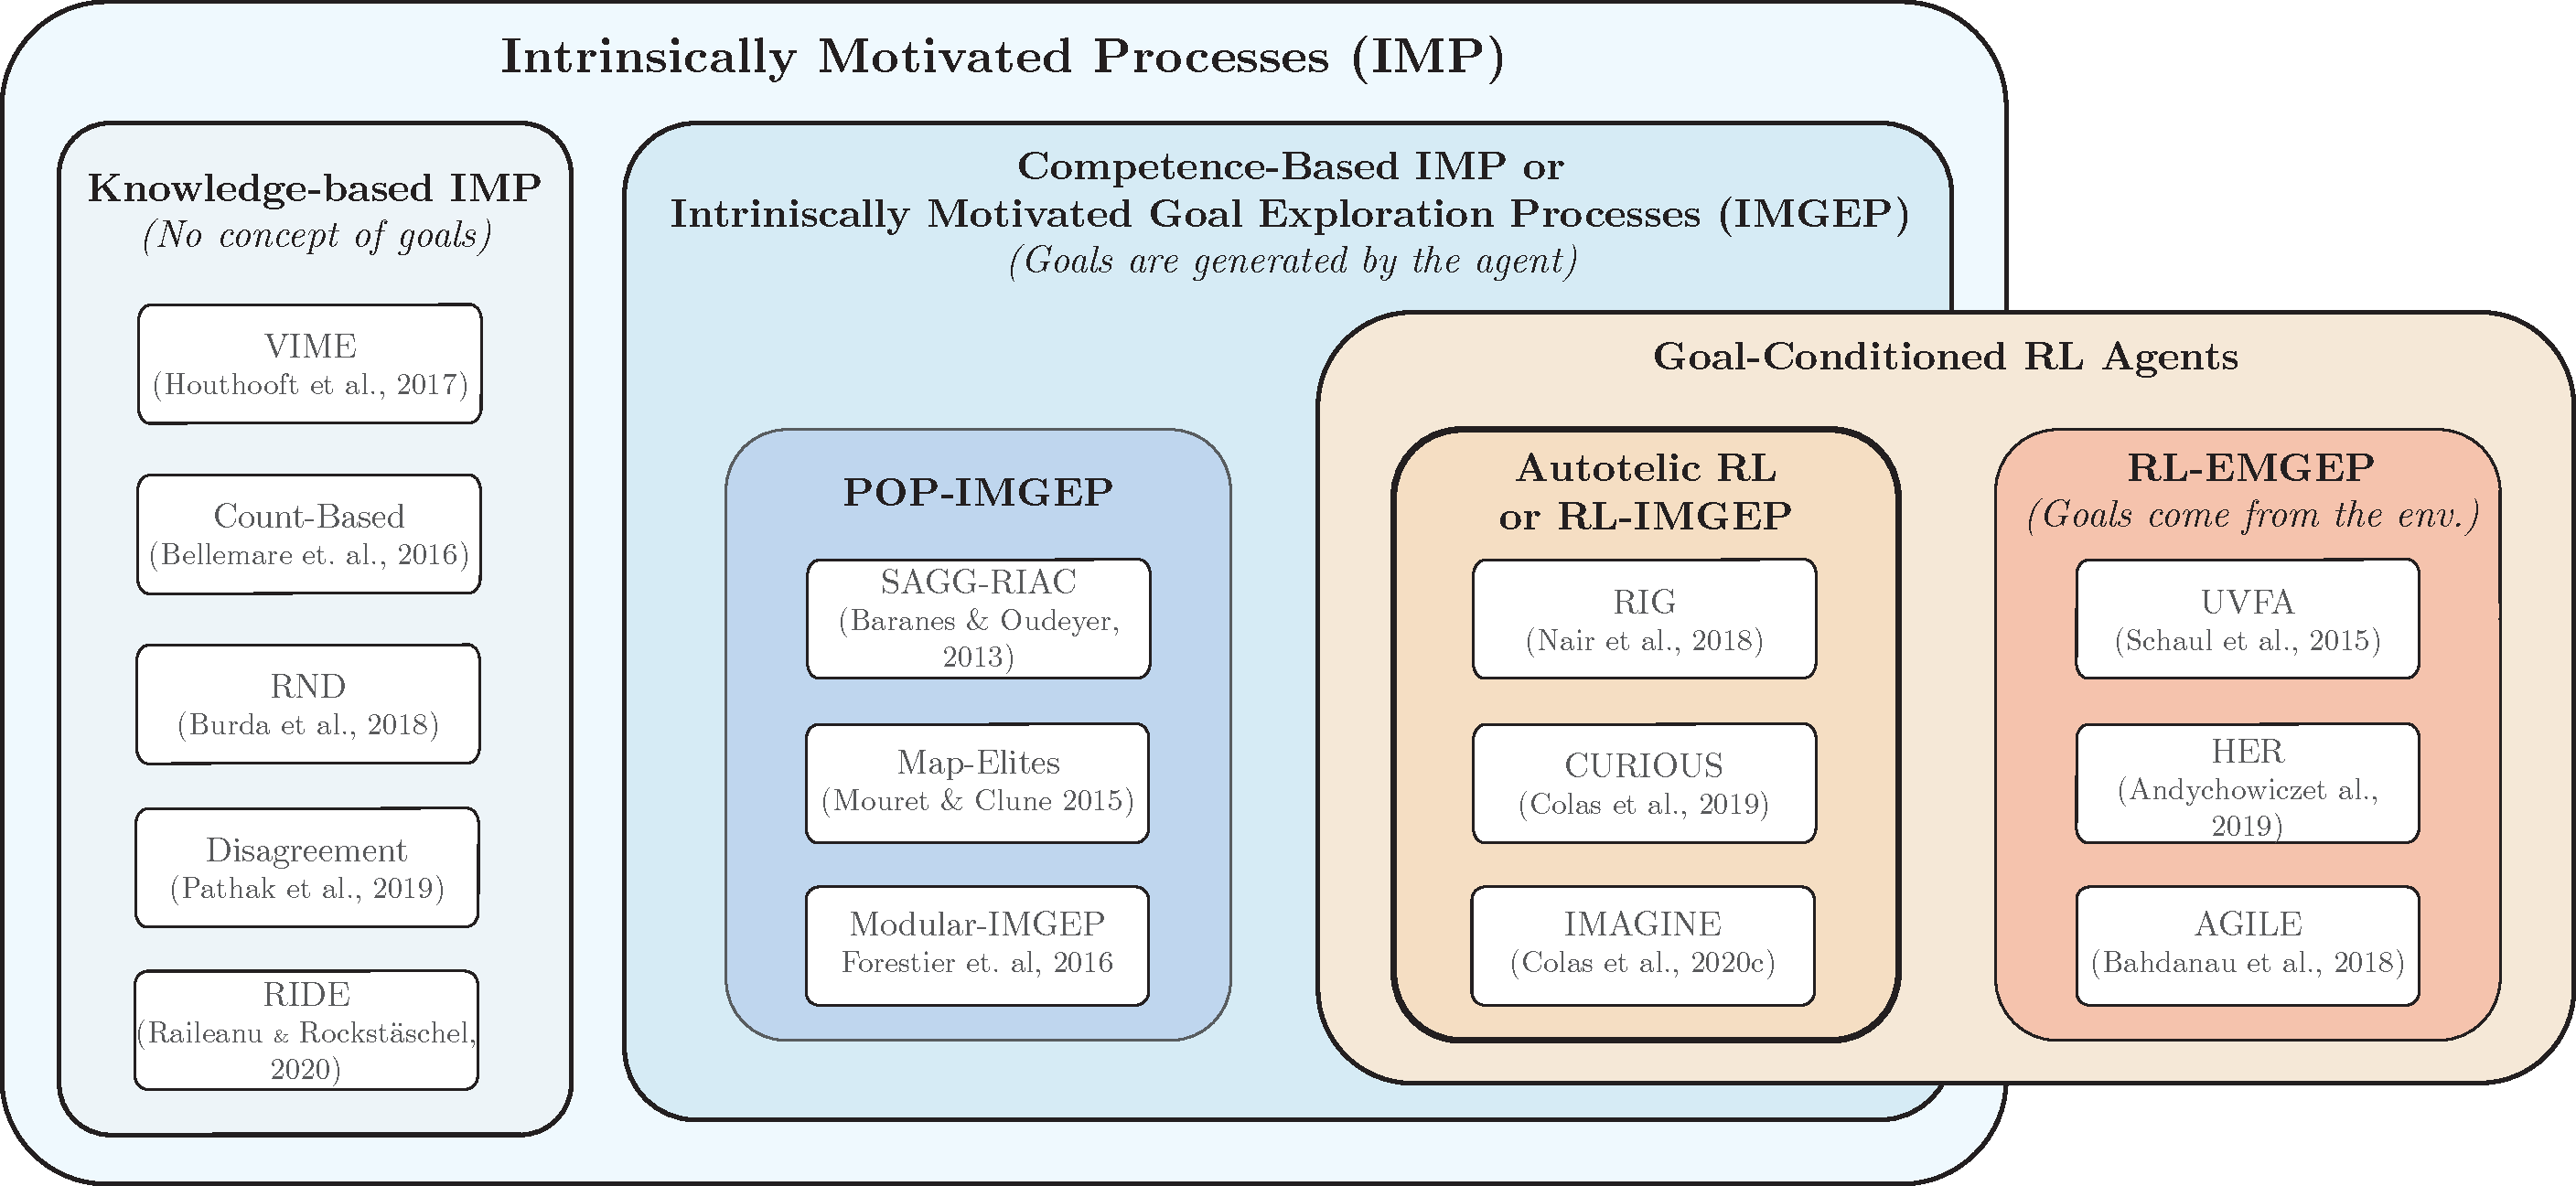
\includegraphics[width=\textwidth]{survey/scope_survey.pdf}
\caption{A typology of intrinsically-motivated and/or goal-conditioned rl approaches. \popimgep, \rlimgep and \rlemgep refer to population-based intrinsically motivated goal exploration processes, \rl-based \imgep and \rl-based externally motivated goal exploration processes respectively. \popimgep, \rlimgep, and \rlemgep all represent goals, but knowledge-based \ims do not. While \imgeps (\popimgep and \rlimgep) generate their own goals, \rlemgeps require externally defined goals. Autotelic agents are \rlimgep: at the intersection of goal-conditioned \rl agents and intrinsically motivated processes that train agents to generate and pursue their own goals with goal-conditioned \rl algorithms.}	
\end{figure}

\paragraph{The Intrinsically Motivated Skills Acquisition Problem}

In the \textit{intrinsically motivated skills acquisition problem}, the agent is set in an open-ended environment without any pre-defined goal and needs to acquire a repertoire of skills. Here, a skill is defined as the association of a goal embedding $z_g$ and the policy to reach it $\Pi_g$. A repertoire of skills is thus defined as the association of a repertoire of goals $\m{G}$ with a goal-conditioned policy trained to reach them $\Pi_\m{G}$. The intrinsically motivated skills acquisition problem can now be modeled by a reward-free \mdp $\m{M}\,=\,\{\m{S},\, \m{A},\, \m{T},\, \rho_0\}$ that only characterizes the agent, its environment and their possible interactions. Just like children, agents must be autotelic, \ie they should learn to represent, generate, pursue and master their own goals.

\begin{figure}[!h]
\centering
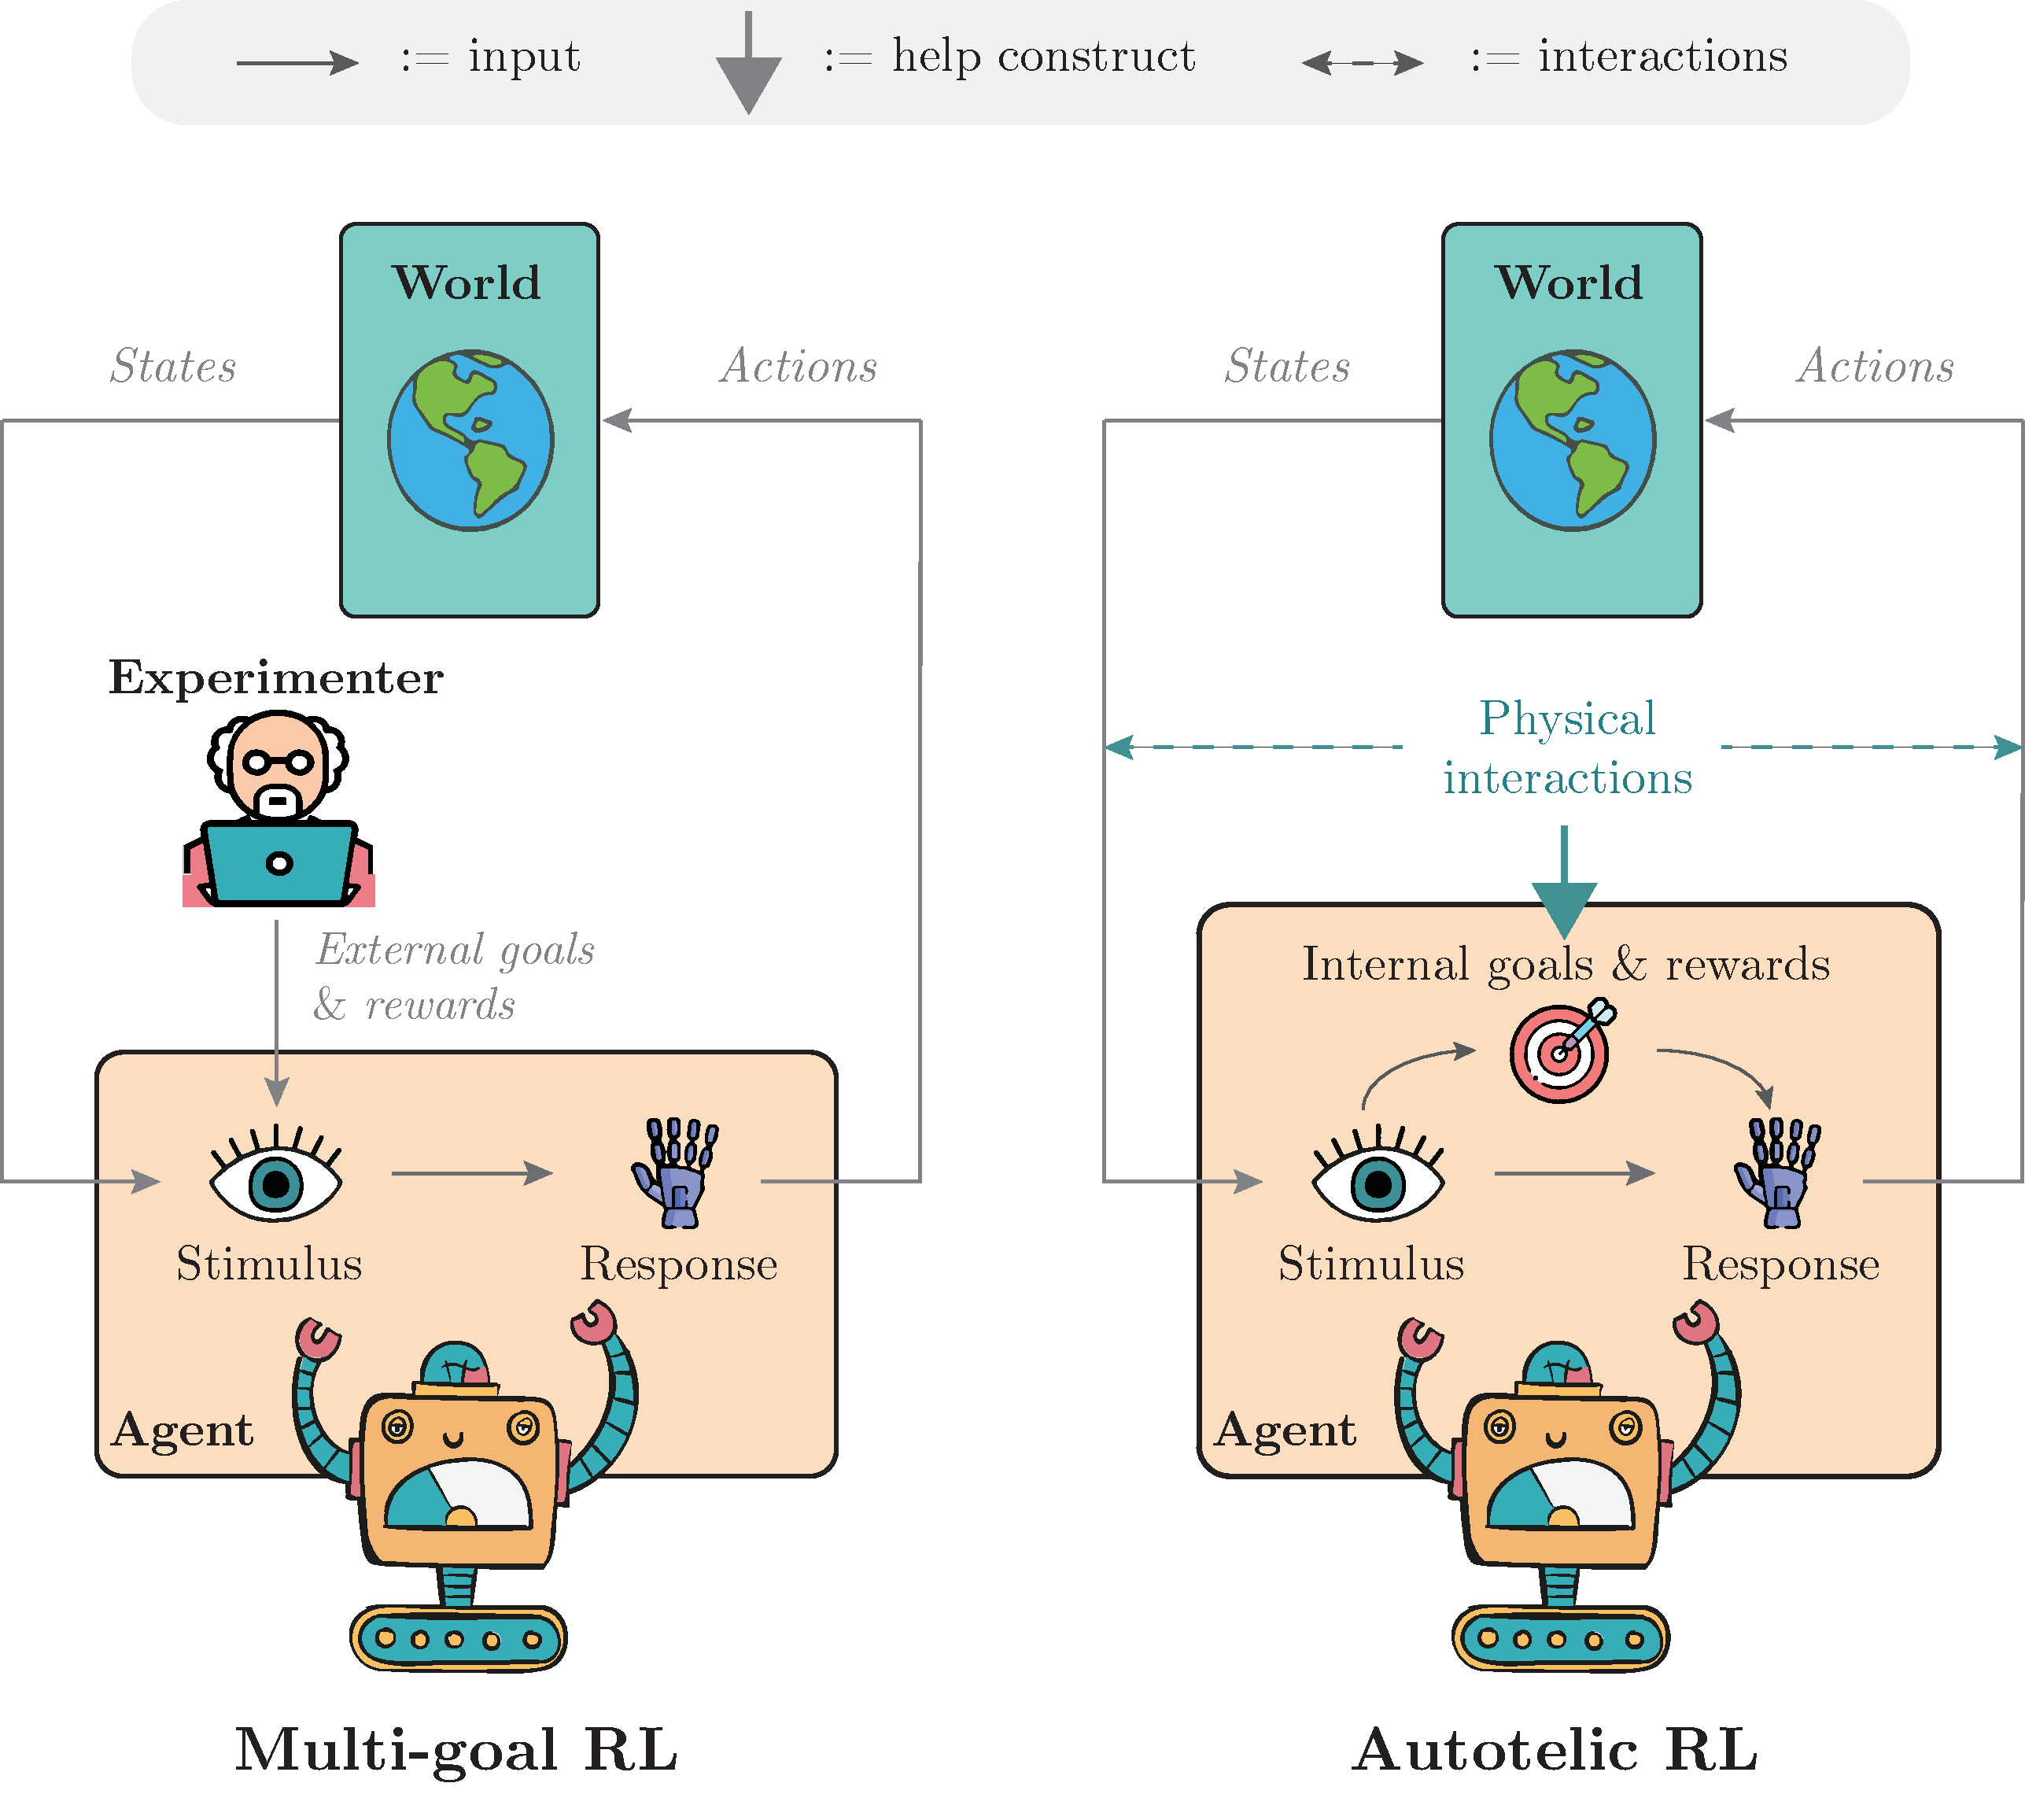
\includegraphics[width=.65\textwidth]{background/autotelic_rl_interactions.pdf}
\caption{}
\end{figure}

\paragraph{Evaluating Autotelic Agents}

Evaluating agents is often trivial in reinforcement learning. Agents are trained to maximize one or several pre-coded reward functions\,---\,the set of possible interactions is known in advance. One can measure generalization abilities by computing the agent's success rate on a held-out set of testing goals. One can measure exploration abilities via several metrics such as the count of task-specific state visitations.

In contrast, autotelic agents evolve in open-ended environments and learn to represent and form their own set of skills. In this context, the space of possible behaviors might quickly become intractable for the experimenter, which is perhaps the most interesting feature of such agents. For these reasons, designing evaluation protocols is not trivial.

The evaluation of such systems raises similar difficulties as the evaluation of task-agnostic content generation systems like Generative Adversarial Networks (\gan) \citep{goodfellow2014generative} or self-supervised language models \citep{devlin2019bert,brown2020language}. In both cases, learning is \textit{task-agnostic} and it is often hard to compare models in terms of their outputs (\eg comparing the quality of \gan output images, or comparing output repertoires of skills in autotelic agents).

One can also draw parallel with the debate on the evaluation of open-ended systems in the field of \textit{open-ended evolution} \citep{hintze_open-endedness_2019,stanley_role_2016,stanley_why_2019}. In both cases, a \textit{good} system is expected to generate more and more original solutions such that its output cannot be predicted in advance. But what does \textit{original} mean, precisely? \citep{stanley_role_2016} argues that subjectivity has a role to play in the evaluation of open-ended systems. Indeed, the notion of \textit{interestingness} is tightly coupled with that of \textit{open-endedness}. What we expect from our open-ended systems, and of our \rlimgep agents in particular, is to generate more and more behaviors that \textit{we} deem interesting. This is probably why the evaluation of content generators often include human studies. Our end objective is to generate interesting artefacts for us; we thus need to evaluate open-ended processes ourselves, subjectively.

Our end goal would be to interact with trained \rlimgep directly, to set themselves goals and test their abilities. The evaluation would need to adapt to the agent's capabilities. As Einstein said \textit{``If you judge a fish by its ability to climb a tree, it will live its whole life believing that it is stupid.''}. \rlimgep need to be evaluated by humans looking for their area of expertise, assessing the width and depth of their capacities in the world they were trained in. This said, science also requires more objective evaluation metrics to facilitate the comparison of existing methods and enable progress. Let us list some evaluation methods measuring the competency of agents via proxies:

\begin{itemize}
    \item \textbf{Measuring exploration:} one can compute task-agnostic exploration proxies such as the entropy of the
    visited state distribution, or measures of state coverage (\eg coverage of the high-level x-y state space in mazes) \citep{goalgan}. Exploration can also be measured as the number of interactions from a set of \textit{interesting} interactions defined subjectively by the experimenter (interactions with objects \citet{imagine}).
    \item \textbf{Measuring generalization:} The experimenter can subjectively define a set of relevant target goals
    and prevent the agent from training on them. Evaluating agents on this held-out set at test time provides a measure of generalization \citep{ruis2020benchmark}, although it is biased towards what the experimenter assesses as \textit{relevant} goals.
    \item \textbf{Measuring transfer learning:} The intrinsically motivated exploration of the environment can be seen as a pre-training phase to bootstrap learning in a subsequent downstream task. In the downstream task, the agent is trained to achieve externally-defined goals. We report its performance and learning speed on these goals. This is akin to the evaluation of self-supervised language models, where the reported metrics evaluate performance in various downstream tasks \citep{brown2020language}. In this evaluation setup, autotelic agents can be compared to task-specific agents. Ideally, autotelic agents should benefit from their open-ended learning process to outperform task-specific agents on their own tasks. This said, performance on downstream tasks remains an evaluation proxy and should not be seen as the explicit \textit{objective} of the skill discovery phase. Indeed, in humans, skill discovery processes do not target any specific future task, but emerged from a natural evolutionary process maximizing reproductive success, see a discussion in \citep{singh2010intrinsically}.
    \item \textbf{Opening the black-box:} Investigating internal representations learned during intrinsically motivated exploration is often informative. One can investigate properties of the goal generation system (\eg does it generate out-of-distribution goals?), investigate properties of the goal embeddings (\eg are they disentangled?). One can also look at the learning trajectories of the agents across learning, especially when they implement their own curriculum learning \citep{goalgan,curious,blaes2019control,pong2019skew,akakzia2020decstr}.
    \item \textbf{Measuring robustness:} Autonomous learning agents evolving in open-ended environment should be robust to a variety of properties than can be found in the real-world. This includes very large environments, where possible interactions might vary in terms of difficulty (trivial interactions, impossible interactions, interactions whose result is stochastic thus prevent any learning progress). Environments can also include distractors (\eg non-controllable objects) and various forms of non-stationarity. Evaluating learning algorithms in various environments presenting each of these properties allows to assess their ability to solve the corresponding challenges.
\end{itemize}


\paragraph{Autotelic RL Agents}

Until recently, the \imgep family was powered by population-based algorithms (\popimgep). The emergence of goal-conditioned \rl approaches that generate their own goals gave birth to a new type of \imgeps: the \rl-based \imgeps (\rlimgep). This section builds on traditional \rl and goal-conditioned \rl algorithms to give a general definition of intrinsically motivated goal-conditioned \rl algorithms (\rlimgep).

\rlimgep are intrinsically motivated versions of goal-conditioned \rl algorithms. They need to be equipped with mechanisms to represent and generate their own goals in order to solve the intrinsically motivated skills acquisition problem, see Figure~\ref{fig:goal_directed_rl}. Concretely, this means that, in addition to the goal-conditioned policy, they need to learn: 1)~to represent goals $g$ by compact embeddings $z_g$; 2)~to represent the support of the goal distribution, also called \textit{goal space} $\m{Z}_\m{G}=\{z_g\}_{g\in\m{G}}$; 3)~a goal distribution from which targeted goals are sampled $\m{D}(z_g)$; 4)~a goal-conditioned reward function $\m{R}_\m{G}$. In practice, only a few architectures tackle the four learning problems above. 

In this survey, \textbf{we call \textit{autotelic} any architecture where the agent selects its own goals (learning problem 3)}. Simple autotelic agents assume pre-defined goal representations (1), the support of the goals distribution (2) and goal-conditioned reward functions (4). As autotelic architectures tackle more of the 4 learning problems, they become more and more advanced. As we will see in the following sections, many existing works in goal-conditioned \rl can be formalized as autotelic agents by including goal sampling mechanisms \textit{within the definition of the agent}. 

With a developmental perspective, one can reinterpret existing work through the autotelic \rl framework. Let us take an example. The \textsc{agent$_{57}$} algorithm automatically selects a parameter to balance the intrinsic and extrinsic rewards of the agent at the beginning of each training episode \citep{badia2020agent57}. The authors do not mention the concept of \textit{goal} but instead present this mechanism as a form of reward shaping technique independent from the agent. With a developmental perspective, one can interpret the mixing parameter as a goal embedding. Replacing the sampling mechanism within the boundaries of the agent, \textsc{agent$_{57}$} becomes autotelic. It is intrinsically motivated to sample and target its own goals; \ie to define its own reward functions (here mixtures of intrinsic and extrinsic reward functions). 

Algorithm~\ref{algo:IMGEP} details the pseudo-code of \rlimgep algorithms. Starting from randomly initialized modules and memory, \rlimgep agents enter a standard \rl interaction loop. They first observe the context (initial state), then sample a goal from their goal sampling policy. Then starts the proper interaction. Conditioned on their current goal embedding, they act in the world so as to reach their goal, \ie to maximize the cumulative rewards generated by the goal-conditioned reward function. After the interaction, the agent can update all its internal models. It learns to represent goals by updating its goal embedding function and goal-conditioned reward function, and improves its behavior towards them by updating its goal-conditioned policy. 

\begin{figure}[!h]
\centering
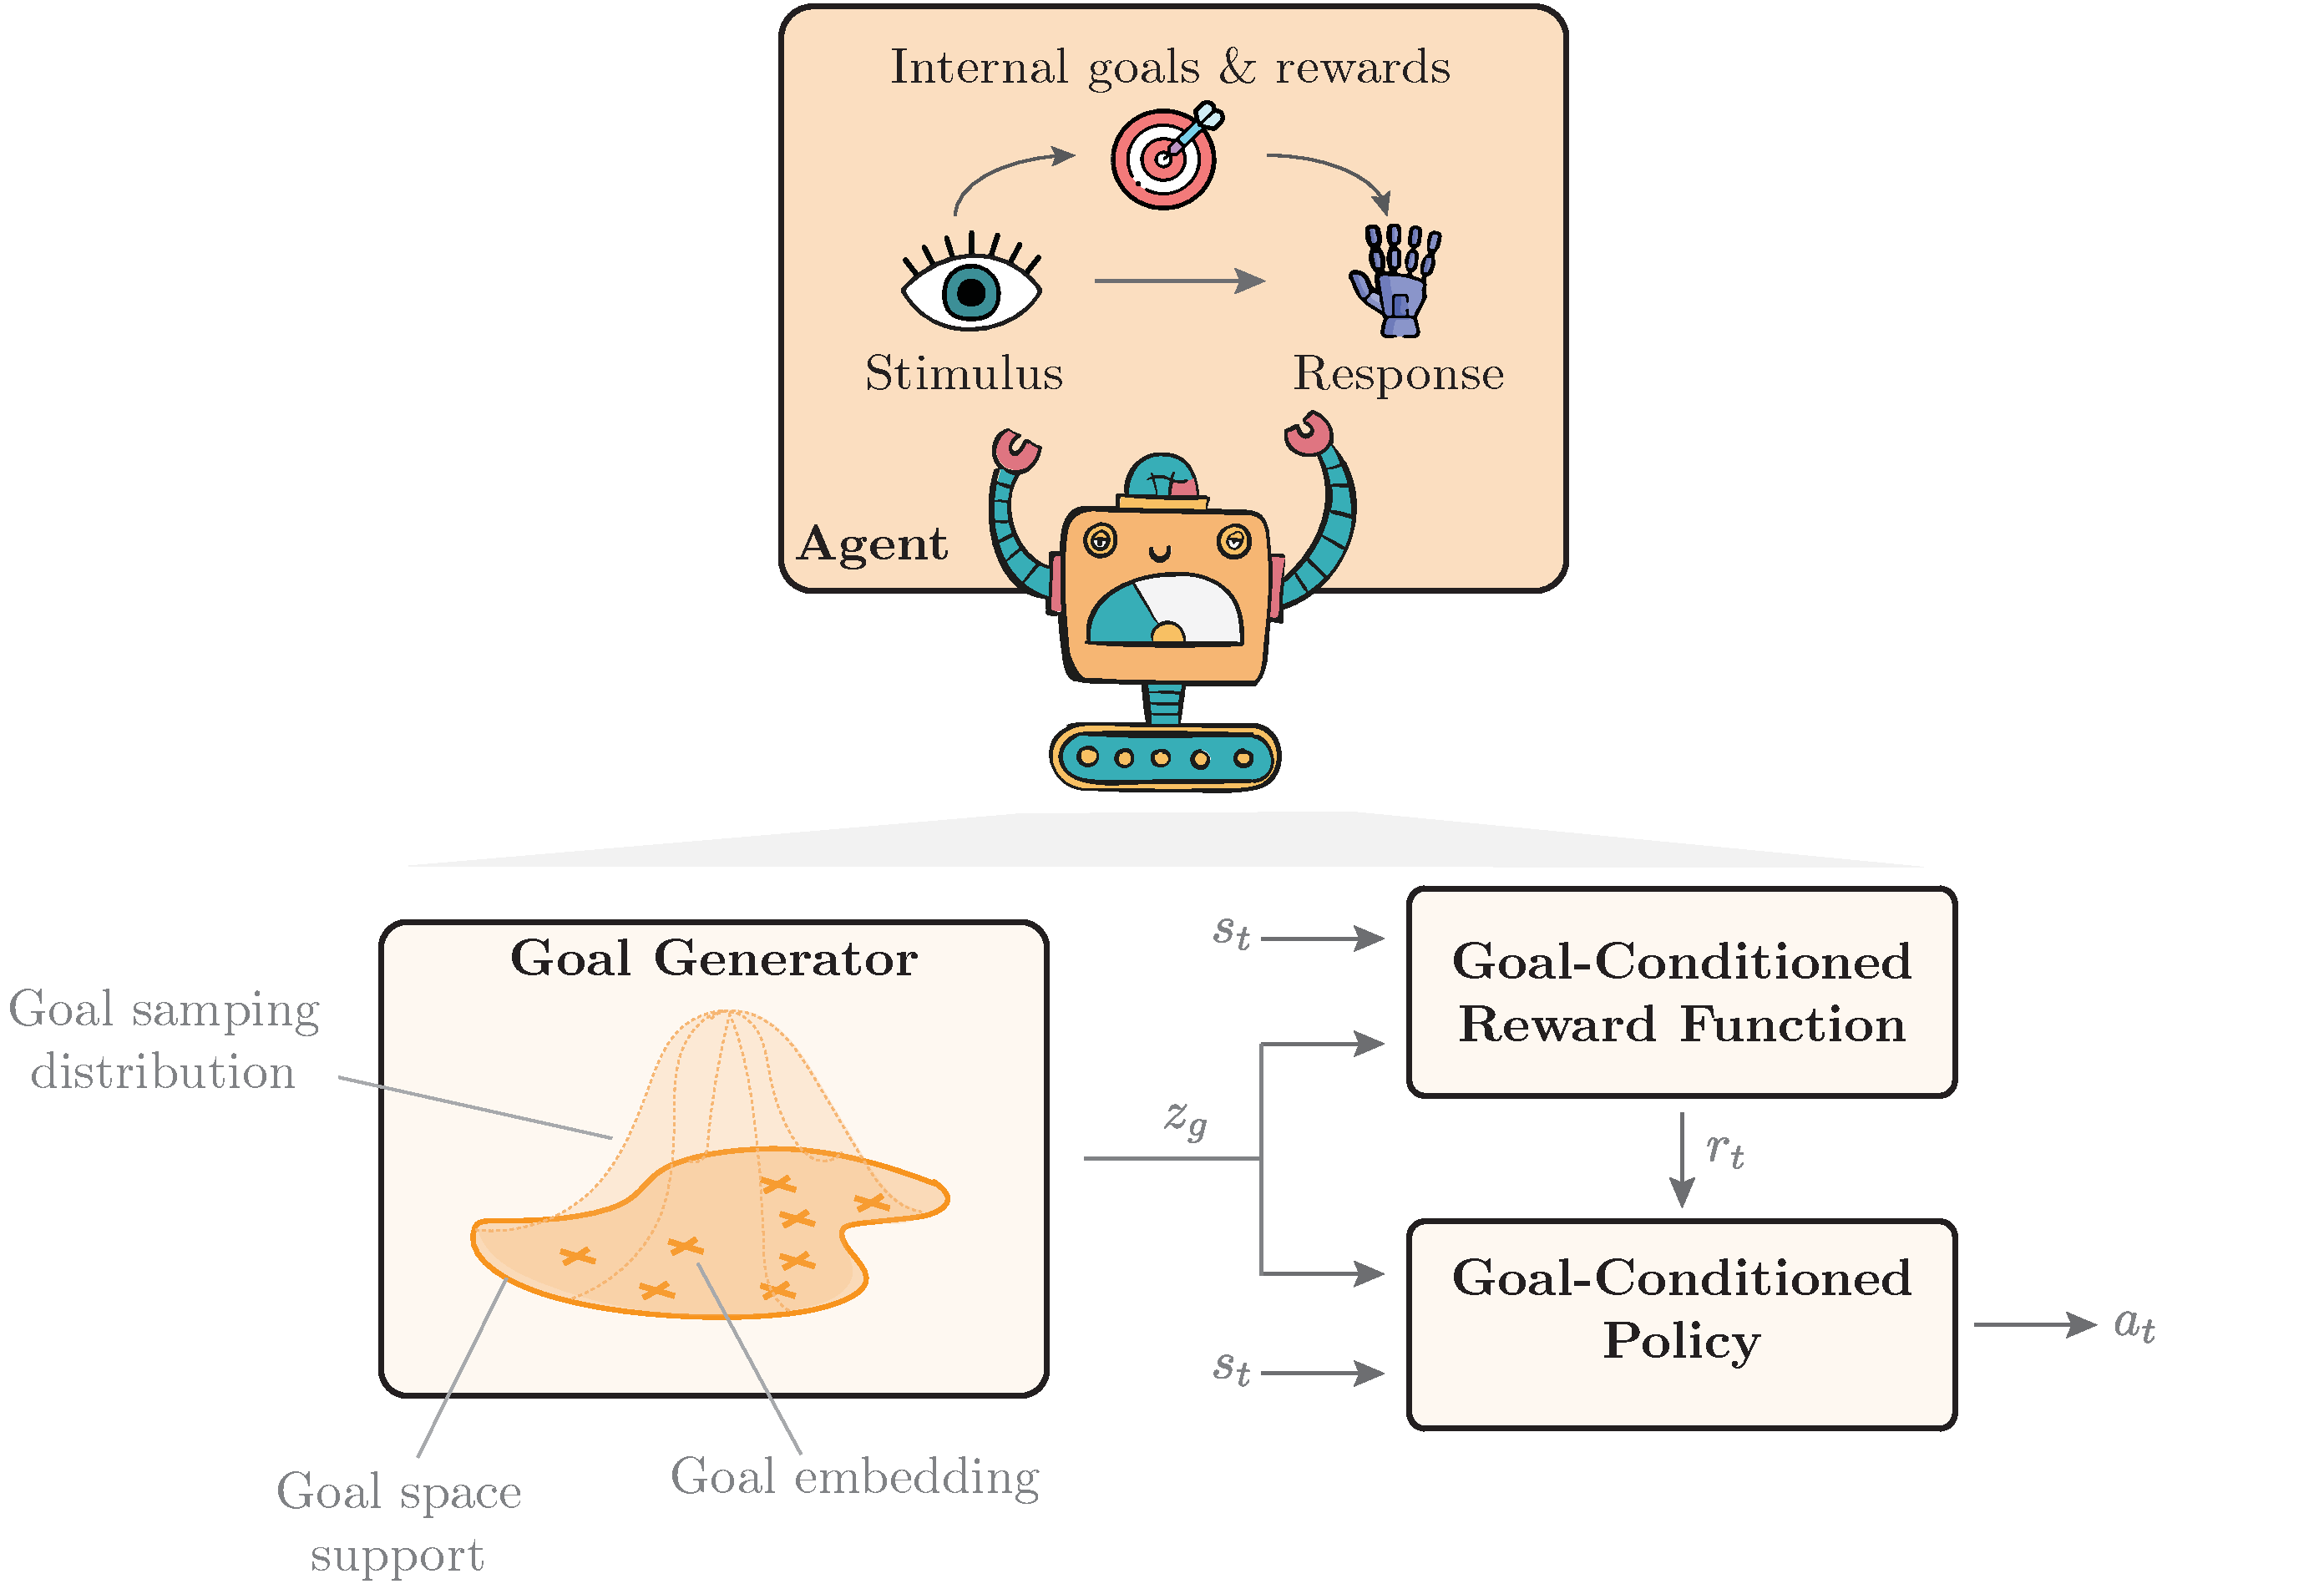
\includegraphics[width=.65\textwidth]{background/inside_autotelic_agent.pdf}
\caption{}
\end{figure}
\noindent\begin{minipage}{\textwidth}
   \centering
   \begin{minipage}{.6\textwidth}
        \begin{algorithm}[H]
            \small
        	\caption{~ Autotelic Agent with RL-IMGEP}
        	\label{algo:IMGEP}
        	\begin{algorithmic}[1]
            	\REQUIRE environment $\m{E}$
            	\STATE \textbf{Initialize} empty memory $\m{M}$,goal-conditioned policy $\Pi_\m{G}$, goal-conditioned reward $R_\m{G}$,goal space $\m{Z}_\m{G}$, goal sampling policy $GS$.
            	
            	\LOOP
            	
%                \LineCommentConttwo{\textit{Observe context}}
                \STATE Get initial state: $s_0 \leftarrow \m{E}$.reset()
%            	\LineCommentCont{\textit{Sample goal}}
            	\STATE Sample goal embedding $z_g=GS(s_0, \m{Z}_\m{G})$.
%            	\LineCommentCont{\textit{Roll-out goal-conditioned policy}}
            	\STATE Execute a roll-out with $\Pi_g=\Pi_\m{G}(\cdot \mid z_g)$
            	\STATE Store collected transitions $\tau=(s,a,s')$ in $\m{M}$.
%            	\LineCommentCont{\textit{Update internal models}}
                \STATE Sample a batch of $B$ transitions: $\m{M}\sim \{(s,a,s')\}_B$.
                \STATE Perform Hindsight Relabelling $\{(s,a,s',z_g)\}_B$.
                \STATE Compute internal rewards $r=R_\m{G}(s,a,s'\mid z_g)$.
            	\STATE Update policy $\Pi_\m{G}$ via \rl on $\{(s,a,s',z_g,r)\}_B$.
            	\STATE Update goal representations  $\m{Z}_\m{G}$. 
            	\STATE Update goal-conditioned reward function $R_\m{G}$. 
            	\STATE Update goal sampling policy $GS$.
            	\ENDLOOP
            	\STATE \Return $\Pi_\m{G}, R_\m{G}, \m{Z}_\m{G}$
        	\end{algorithmic}
        \end{algorithm}
   \end{minipage}
   \hspace{0.2cm}
   \begin{minipage}{.37\textwidth}
  \textbf{ } \\
  \\
        \centering
        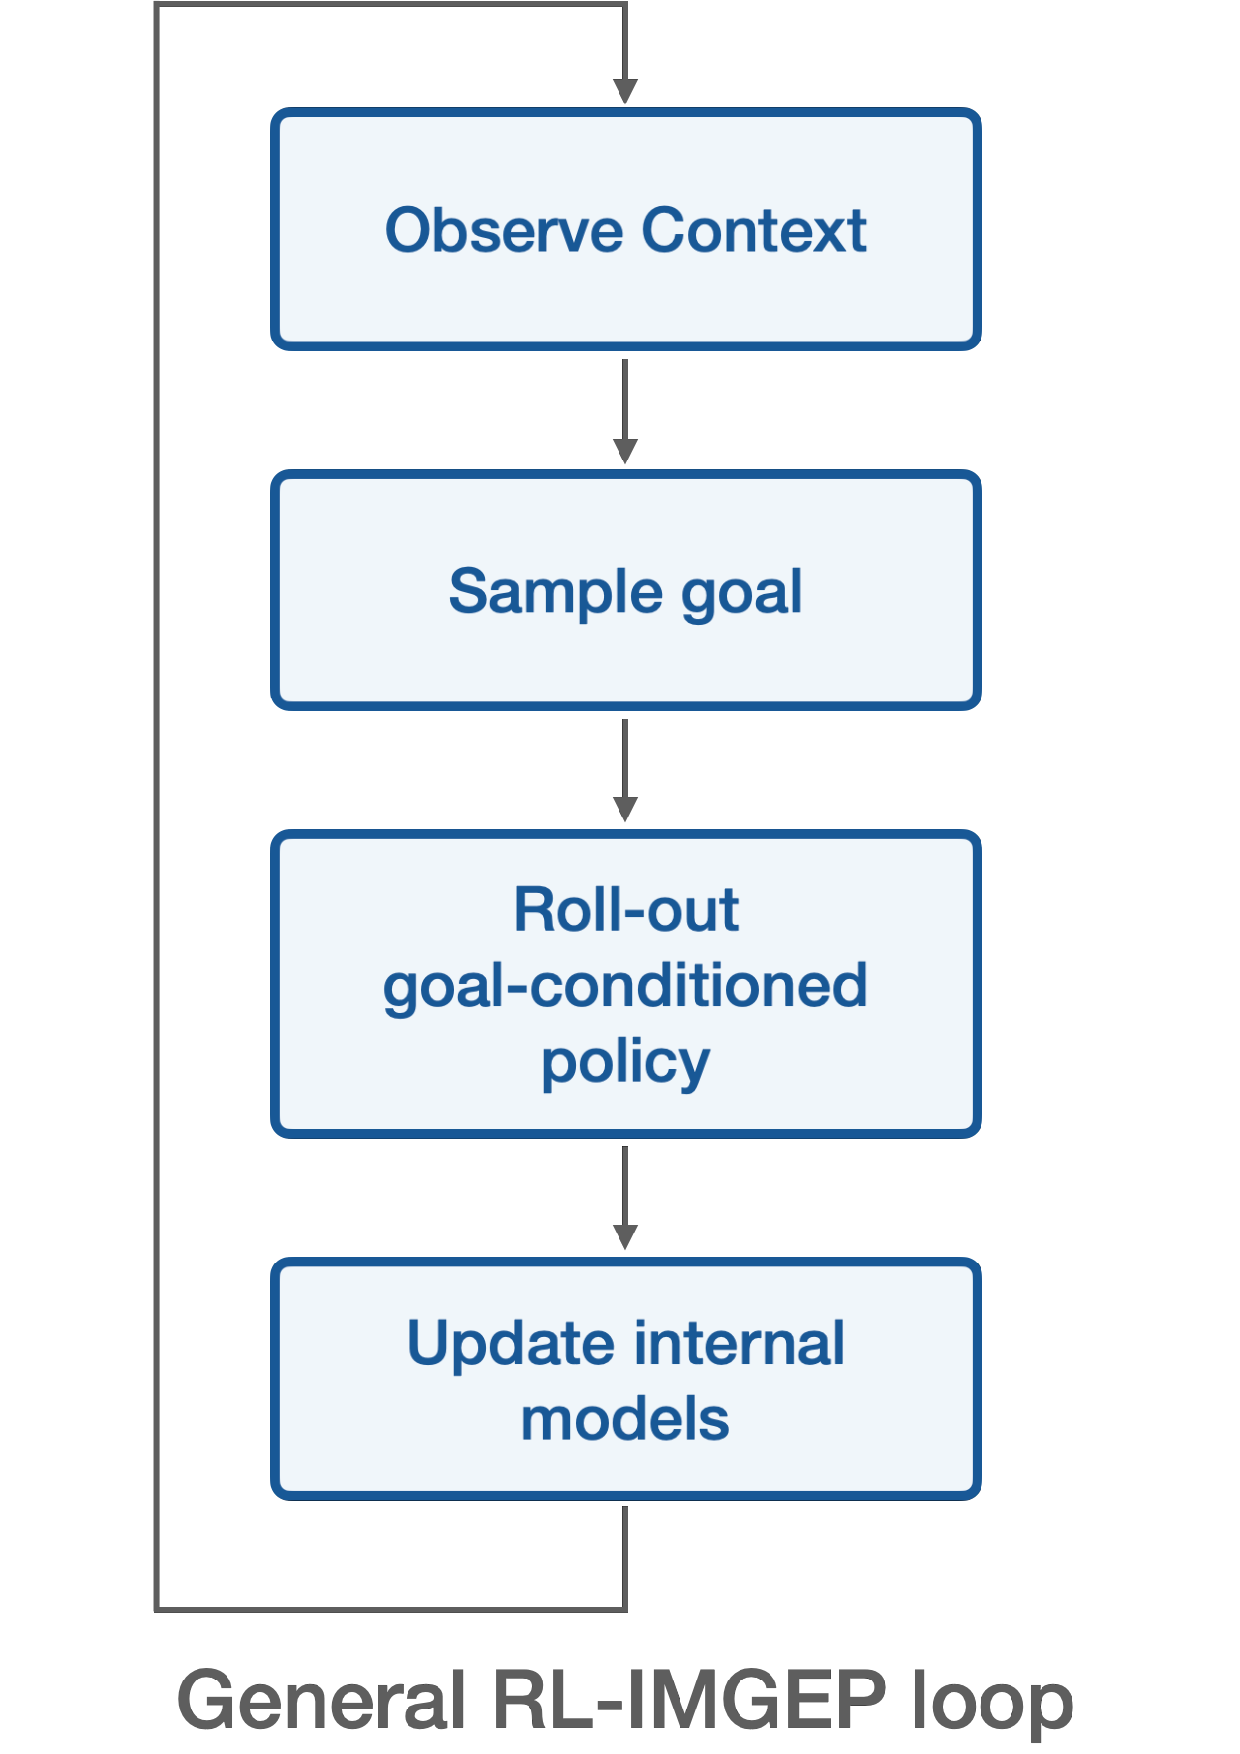
\includegraphics[width=0.9\textwidth]{survey/loop-algo.pdf}
    \end{minipage}
   \label{fig:test}
\end{minipage}
    



\todo{adjust this} This surveys focuses on the mechanisms specific to \rlimgep agents, \ie mechanisms that handle the representation, generation and selection of goals. These mechanisms are mostly orthogonal to the question of how to reach the goals themselves, which often relies on existing goal-conditioned algorithms, but can also be powered by imitation learning, evolutionary algorithms or other control and planning methods. Section~\ref{sec:survey_goal_rep} first presents a typology of goal representations used in the literature, before Sections~\ref{sec:survey_learning_goal_rep}~and~\ref{sec:survey_generation} cover existing methods to learn to represent and prioritize goals respectively.




